\documentclass[lettersize,journal]{IEEEtran}
\usepackage{amsmath,amsfonts}
\usepackage{algorithmic}
\usepackage{algorithm}
\usepackage{array}
\usepackage[caption=false,font=normalsize,labelfont=sf,textfont=sf]{subfig}
\usepackage{subcaption}
\usepackage{textcomp}
\usepackage{stfloats}
\usepackage{url}
\usepackage{verbatim}
\usepackage{graphicx}
\usepackage{cite}
\hyphenation{op-tical net-works semi-conduc-tor IEEE-Xplore}
% updated with editorial comments 12/2/2022

\begin{document}

\title{Journal DAO: \\ User-Incentivized Autonomous Decentralized Scientific Publishing in Web3}

\author{Tai Jiang, Rui Qin,~\IEEEmembership{Member, IEEE}, Yuhang Liu, \\
 Fei-YueWang,~\IEEEmembership{Fellow,~IEEE}.
        % <-this % stops a space
\thanks{This work was supported by the Science and Technology Development Fund of Macau SAR under Grant 0093/2023/RIA2 and  Grant 0050/2020/A1.}% <-this % stops a space
\thanks{Manuscript received February 15, 2023; revised February 15, 2023.}
\thanks{Tai Jiang is with the Department of Engineering Science, Faculty of Innovation Engineering, Macau University of Science and Technology, Macao, 999078, China (e-mail: jiangtai20@mails.ucas.ac.cn).}
\thanks{Rui Qin is with the State Key Laboratory for Management and Control of Complex Systems and the State Key Laboratory of Multimodal Artificial Intelligence Systems, Institute of Automation, Chinese Academy of Sciences, Beijing 100190, China (e-mail: rui.qin@ia.ac.cn).}
\thanks{Yuhang Liu is with the State Key Laboratory for Management and Control of Complex Systems, Institute of Automation, Chinese Academy of Sciences, Beijing 100190, China, and also with the School of Artificial Intelligence, University of Chinese Academy of Sciences, Beijing 100049, China (e-mail: liuyuhang21@mails.ucas.ac.cn).}
\thanks{Fei-Yue Wang is with the State Key Laboratory for Management and Control of Complex Systems, Chinese Academy of Sciences, Beijing 100190, China, and also with the Macao Institute of Systems Engineering, Macau University of Science and Technology, Macao 999078, China (e-mail: feiyue.wang@ia.ac.cn).}

}

% The paper headers
\markboth{Journal of \LaTeX\ Class Files,~Vol.~14, No.~8, February~2023}%
{Shell \MakeLowercase{\textit{et al.}}: A Sample Article Using IEEEtran.cls for IEEE Journals}

% \IEEEpubid{0000--0000/00\$00.00~\copyright~2021 IEEE}
% Remember, if you use this you must call \IEEEpubidadjcol in the second
% column for its text to clear the IEEEpubid mark.

\maketitle

\begin{abstract}
The emergence of Web3.0 signifies a significant evolution in the Internet landscape, emphasizing decentralization, openness, and user control over data. This paper outlines the key characteristics of Web3.0, including a decentralized network architecture, the application of smart contracts, and data privacy protection. Leveraging blockchain technology, the paper discusses how it can facilitate the authenticity, security, and traceability of paper data, offering a novel perspective on ownership and governance. Through the decentralized autonomous organization (DAO) framework, a more just, transparent, and open organizational structure can be realized, bringing new governance models to the academic research domain. This structure emphasizes equitable stakeholder participation, fostering collaborative development within the academic community. Lastly, the paper presents the implementation of a DAO framework called DeSCI, designed to streamline the lifecycle of scholarly articles, including submission, peer review, downloading, and citation processes, all securely recorded on the blockchain. By utilizing Non-Fungible Tokens (NFTs), the framework introduces a sophisticated incentive structure for authors, reviewers, and users. The incorporation of NFTs ensures a novel approach to fostering a decentralized and incentivized ecosystem for academic publishing, marking a substantial advancement in the realm of scholarly communication.
%Web3.0的出现标志着互联网领域的显著演变,强调去中心化、开放性和用户对数据的控制。本文首先勾勒了Web3.0的关键特征,包括分散式网络架构、智能合约的应用以及数据隐私的保护。在区块链技术的背景下,本文讨论了如何利用区块链的不可变性和透明性促进论文数据的真实性、安全性和可追溯性,为所有权和治理提供了新的视角。通过分散自治组织(DAO)框架,可以实现更公正、透明和开放的组织结构,为学术研究领域带来新的治理模式。这种结构强调了利益相关者的更公平参与,促进了学术界的协作发展。最后,本文介绍了一个名为DeSCI的DAO框架的实现,旨在简化学术文章的生命周期,包括提交、同行评审、下载和引用过程,所有这些过程都在区块链上安全记录。通过使用非同质化代币(NFTs),该框架为作者、审稿人和用户引入了一种复杂的激励结构。NFTs的引入确保了促进学术出版的分散化和激励性生态系统的新方法,标志着学术交流领域的重大进展。
\end{abstract}


\begin{IEEEkeywords}
DAO, smart contract, decentralized autonomous organizations, decentralized funding, decentralized science, DeSci, parallel DeSci, Web3
\end{IEEEkeywords}

\section{Introduction \label{sec:introduction}}
% 第一段:目前期刊运行存在的问题与挑战
% 第二段:新技术的发展为期刊运行提供了哪些发展机遇
% 第三段:简述已有的期刊变革方面的研究
% 第四段:已有研究中尚存在的问题,本文的主要工作
% 第五段:本文的结构安排

%不需要介绍学术出版行业发展的历程。
%第一段只需要介绍学术出版行业目前面临哪些严峻问题(一定要列本文中要解决的那些问题);First, .... Second,.... Third,....

%第二段综述学术出版领域已有哪些文献采用这些新技术去解决第一段所列出的问题。讲完这些文献之后,要对以上文献进行述评,要表述出这些文献只是从XX方面对这些问题进行了初步探讨,并没有真正解决以上问题,目前也没有针对以上问题的一套完整有效解决方案。

%第三段简要介绍区块链、DAO等新技术的出现给学术出版业带来哪些发展机遇。详细介绍这些新技术的哪些特性可以解决学术出版行业的哪些问题。

%第四段介绍本文的工作和贡献。采用总分总的形式,先总体介绍本文的主要贡献:将区块链、DAO等新技术应用于学术出版领域,提出Journal DAO,利用区块链和DAO的哪些特性,为学术出版行业面临的哪些问题提供有效解决方案。再分别介绍本文的具体贡献,分三点列出,第一点提出Journal DAO的研究思路与框架,第二点提出Journal DAO的模型,第三点给出一个案例。最后总结一句本文工作的重要性。

%第五段简要介绍本文的结构安排。第二节。。。,第三节。。。。,第四节。。。。,第五节。。。。,很简短地介绍即可,本段内容大概四五行。


\IEEEPARstart{A}{cademic} paper face several challenges recently, including peer review, authenticity, and copyright. 
Firstly, lack of complete transparency in the review process. The traditional peer review system, often conducted anonymously, may not always ensure fairness and impartiality. The identities of the reviewers and their feedback are typically kept confidential, making it difficult for authors to understand the rationale behind decisions and address any potential biases. This lack of transparency can undermine the credibility and integrity of the review proces. 
Secondly, While authors are credited with the authorship of a paper, they often lack control over the various data associated with it. In many cases, the ownership and control of data reside with the publishers or electronic journal databases. This poses a challenge to authors in terms of retaining their rights and having the ability to decide on data sharing, data transformation, or deriving benefits from their own research. This lack of control over their own data not only hampers their ability to fully utilize and leverage their research but also limits their potential for collaborations and further advancements in their field. 
Thirdly, Academic papers rely on data to support their findings and conclusions. However, the current system often restricts the ability of authors to share or collaborate on their data. The data associated with a paper is typically stored within electronic journal databases or controlled by publishers, limiting the author's autonomy to decide on sharing, collaboration, or commercialization opportunities. This restriction hampers the progress of research as it impedes the free flow of knowledge and inhibits potential collaborations among researchers. Additionally, it prevents authors from fully benefiting from their own research, restricting the potential for further discoveries and advancements that could benefit the scientific community as a whole. 
These challenges highlight the need for reforms in the academic publishing system to address issues related to transparency, author rights protection, and data sharing. Implementing new technologies, such as blockchain\cite{swan2015blockchain}, could potentially provide solutions to these problems by ensuring transparency in the review process, protecting author rights, and facilitating data sharing and collaboration in a secure and decentralized manner \cite{mougayar2016business}.
%1. 透明度:当前学术论文面临的一个主要问题是审稿过程缺乏完全的透明度。传统的同行评审系统往往是匿名进行的,不能始终保证公正和客观性。审稿人的身份和评审意见通常是保密的,这使得作者难以了解决策背后的理由并解决潜在的偏见。透明度的缺乏可能损害审稿过程的可信度和完整性。
%2. 作者权益保护:虽然作者被认可为论文的作者,但他们往往无法控制与论文相关的各种数据。在许多情况下,数据的所有权和控制权掌握在出版商或电子期刊数据库手中。这对作者来说是一个挑战,因为他们缺乏保护自己权益和决定数据共享、数据转化或从自己的研究中获益的能力。对自己数据缺乏控制不仅限制了他们充分利用和发挥研究的能力,也限制了他们在领域内进行合作和进一步发展的潜力。
%3. 数据共享与合作:学术论文依赖数据来支持其发现和结论。然而,目前的系统往往限制了作者分享或合作使用数据的能力。与论文相关的数据通常存储在电子期刊数据库内或由出版商控制,限制了作者决定共享、合作或商业化机会的自主权。这种限制阻碍了研究的进展,因为它阻碍了知识的自由流动,并抑制了研究人员之间的潜在合作。此外,它还阻碍了作者充分从自己的研究中获益的能力,限制了进一步发现和进展对整个科学界的潜在益处。
%这些问题突显了学术出版系统需要改革,以解决透明度、作者权益保护和数据共享等问题。采用新技术,如区块链,可能能够提供解决方案,通过确保审稿过程的透明度、保护作者权益以及促进安全和去中心化的数据共享和合作。








Decentralized Autonomous Organization (DAO) have emerged as a disruptive and transformative innovation in the realm of organizational governance. Built on the foundation of blockchain technology and smart contracts, DAOs present a novel approach to decision-making, fund management, and community governance. Unlike traditional hierarchical structures, DAOs operate without the need for central authorities, relying on transparent and automated processes governed by code and consensus \cite{buterin2014next}.
The concept of DAOs originated from the desire to create decentralized and trustless organizations that are not bound by geographical limitations or intermediaries \cite{wang2019decentralized}. DAOs leverage the decentralized nature of blockchain technology to establish a peer-to-peer network where  every participant(authors, reviewers and readers...) can share research artilces resources. By utilizing smart contracts, DAOs can execute predefined rules, eliminating the need for intermediaries or third-party oversight and significantly reducing human intervention, thereby ensuring objectivity and efficiency in every step of the process.
One of the key distinguishing features of DAOs is their ability to provide a transparent and auditable decision-making process \cite{kaal2021decentralized}. By recording all transactions and actions on a blockchain, DAOs ensure that every participant has access to the same set of information, promoting transparency and accountability. This transparency also extends to the allocation and management of funds, as DAOs enable token holders to collectively govern and distribute resources based on predefined rules and consensus mechanisms.
% 去中心化自治組織(DAO)已成為組織治理領域的顛覆性和變革性創新。 DAO 建立在區塊鏈技術和智能合約的基礎上,為決策、資金管理和社群治理提供了一種新穎的方法。與傳統的層級結構不同,DAO 的運作不需要中央機構,而是依賴由程式碼和共識管理的透明和自動化流程。
%DAO 的概念源于创建不受地理限制或中介机构约束的去中心化和去信任组织的愿望。 DAO 利用区块链技术的去中心化特性建立一个点对点网络,作者、审稿人、读者共享论文资源。通过使用智能合约,DAO 可以执行预定义的规则,消除中介或第三方监管,极大减少人为因素,让每一步操作客观有效。
%DAO 的主要显着特征之一是它们能够提供透明且可审计的决策流程。通过在区块链上记录所有交易和操作,DAO 可确保每个参与者都能访问同一组信息,从而提高透明度和问责制。这种透明度还延伸到了资金的分配和管理,因为 DAO 使代币持有者能够根据预定义的规则和共识机制集体管理和分配资源。


blockchain-based smart contracts have received increasing attention in academic circles,Mainly distributed in security, privacy, software engineering, applications, performance, scalability, and other smart contract-related topics \cite{8756390}. 
The current distribution and management processes in open journal systems are plagued by inadequate security, leading to issues such as unauthorized replication and dissemination of research papers. However, the implementation of blockchain technology has addressed these concerns by enhancing the security of electronic journal distribution and management. This approach brings significant benefits: Firstly, more precise and error-free distribution of e-journals within open journal systems. Secondly, improved reputation and increased trust in the open journal system. Lastly, safeguarding the management process of papers, protecting both soft and hard copies of journals from potential hacker threats. By utilizing blockchain technology, the security and efficiency of electronic journal distribution and management are significantly improved \cite{agustin2020blockchain}.
InterPlanetary File System (IPFS) and blockchain technology ensure the authenticity of online publications by storing them on a decentralized IPFS network and verifying their information through the blockchain, ensuring trust and reliability. This approach effectively addresses the challenges related to security and privacy in online publications \cite{nizamuddin2018ipfs}.
The traditional scientific publishing system faces numerous challenges, including high publication costs, slow and biased peer review processes, copyright held by publishers, lack of rewards for contributors, and limited connectivity among researchers. By leveraging decentralized blockchain-based technology, creating a scientific publishing platform can address these issues. This platform utilizes Ethereum smart contracts to expedite the publication process, reduce biases in peer review, and lower publication costs. The model also enhances the quality of scientific research by incorporating new functionalities during the publishing process. The system increases the number of publishers, ensuring complete traceability throughout the publication process, and making scientific papers accessible to anyone for a nominal fee. Additionally, the system adopts a decentralized model for journals and integrates scientific papers with relevant data or datasets. Editors, reviewers, and cited authors are also rewarded \cite{becstacs2023novel}. The system is implemented using the Ethereum Virtual Machine (EVM), which includes frontend, middleware, and backend components. When an author submits a manuscript for evaluation, the system automatically identifies the most suitable editors and reviewers. After the publication process concludes, editors, reviewers, cited authors, and other contributors receive cryptocurrency rewards based on system tokens.
%基于区块链的智能合约在学术界引起了越来越多的关注,主要分布在安全、隐私、软件工程、应用、性能与可扩展性以及其他与智能合约相关的主题。
%目前开放期刊系统中的分发和管理过程存在安全性不足的问题,容易出现论文被复制和传播给不负责任的人的情况。使用区块链技术来维护电子期刊分发和管理过程的安全性,实现了以下3个方面的好处:(1)在开放期刊系统中,电子期刊的分发更加精确,没有错误;(2)开放期刊系统的声誉得到提升,增加了信任感;(3)管理论文的过程按照规定进行,保护了期刊的软拷贝和硬拷贝免受黑客威胁。
%IPFS和区块链技术可以确保在线出版物的真实性,将出版物存储在去中心化的IPFS网络上,并通过区块链验证其信息,以确保信任和可靠性。这种方法解决了在线出版物安全和隐私方面的挑战。
%传统的科学出版系统存在许多问题,如高昂的出版成本、缓慢和有偏见的评审过程、由出版商持有的版权、缺乏对贡献者的奖励以及研究人员之间缺乏联系等。应用去中心化的基于区块链的技术,创建科学出版平台可以解决这些问题。该平台使用以太坊智能合约加速出版过程,减少评审过程中的偏见,并降低出版成本。该模型还通过在出版过程中添加新的功能来提高科学研究的质量。该系统增加了出版商的数量,使出版过程完全可追溯,并使科学论文对任何人都可用,只需支付少量费用。此外,该系统为期刊提供了去中心化模型,并将科学论文与相关数据或数据集集成在一起。编辑、评审人员和引用作者也会得到奖励。该系统使用以太坊虚拟机(EVM)实现,包括前端、中间件和后端。当作者提交一篇稿件进行评估时,系统会自动找到最合适的编辑和评审人员。出版过程结束后,编辑、评审人员、引用作者和其他贡献者将获得基于系统代币的加密货币作为奖励。

The application of blockchain technology in intelligent journal has the potential to revolutionize data transparency and ensure its authenticity. By leveraging smart contracts, the reliability of data can be guaranteed, eliminating the need for third-party oversight. The framework of a DAO offers a higher level of scalability and addresses not only individual functionalities but the system as a whole.
Recent research has demonstrated the feasibility of DAO applications in automating the peer review process and providing incentives to authors, reviewers, and cited authors, thereby fostering a self-sustaining publication ecosystem. While the adoption of DAO and other blockchain applications has become widespread, many implementations have remained largely theoretical, focusing on the concept of self-governance.
However, to truly realize the potential of DAOs, an appropriate and robust incentive mechanism is crucial. Without it, the token issuance within the organization would lack practical significance. This paper aims to explore the incentive mechanisms of DAOs, specifically from the perspective of journal readers, in order to achieve a fully autonomous and economically sustainable DAO ecosystem \cite{ding2022desci}.
By examining the reader's role in the DAO ecosystem, we can delve deeper into the design and implementation of effective incentive mechanisms. This research strives to contribute to the understanding of DAOs and their potential to transform the publication industry, enabling a seamless integration of blockchain technology and fostering a self-governing and economically viable ecosystem.
% 将区块链技术应用于智能杂志,可以彻底改变数据的透明性,并确保其真实性。通过利用智能合约,数据的可靠性得以保证,不再需要第三方监管。去中心化自治组织(DAO)的框架提供了更高层次的可扩展性,不仅解决了单个功能点的问题,而是整个系统的运作。最近的研究表明,DAO应用可以自动化审稿流程,并为作者、审稿人和引用者提供激励,从而实现论文发布的自我管理。尽管DAO和其他区块链应用已经广泛应用,但大多数实现仍然停留在理论层面的自治概念。
%然而,要真正实现DAO的潜力,一个适当且健全的激励机制至关重要。否则,组织内部代币的发行将缺乏实际意义。本文旨在从读者的角度探索DAO的激励机制,以实现完全自治和经济可持续的DAO生态系统。
%通过研究读者在DAO生态系统中的角色,我们可以深入探讨有效激励机制的设计和实施。本研究旨在为我们对DAO的理解和其改变出版行业潜力的贡献,实现区块链技术的无缝集成,推动自我管理和经济可行的生态系统的发展。


% 本文首先会先介绍一下journal dao的框架,包含概念以及运行流程,以及跟现在传统的对比。然后会介绍激励机制的设计和实施。最后会用实验结果验证其效果。
Section \ref{sec:framework}, this paper begins by providing an in-depth introduction to the framework of Journal DAO, including its concepts, operational processes, and a comparative analysis with traditional approaches. 
Section \ref{sec:mechanism}, it delves into the design and implementation of the incentive mechanism within Journal DAO. This section explores the various factors considered in designing the incentive structure, such as rewarding authors, reviewers, and cited authors based on their contributions to the publication process. Additionally, it discusses the integration of token-based incentives to foster motivation and participation among stakeholders.
Section \ref{sec:performance}, subsequently, it presents experimental results to validate the effectiveness of the implemented incentive mechanism in Journal DAO. Through a rigorous evaluation and analysis, the outcomes highlight the impact of the incentive structure on the overall performance, efficiency, and engagement of participants within the system.
Section \ref{sec:conclusion}, the paper concludes with a conclusion and outlook.
%本论文首先详细介绍了Journal DAO的框架,包括其概念、运行流程以及与传统方法的对比。
%在框架概述之后,论文深入探讨了Journal DAO内部激励机制的设计和实施。这一部分探讨了设计激励结构时考虑的各种因素,例如基于作者、审稿人和被引作者在出版过程中的贡献进行奖励。此外,还讨论了通过基于代币的激励促进参与者的积极性和参与度。
%随后,论文呈现了实验结果,验证了Journal DAO实施的激励机制的有效性。通过进行严格的评估和分析,结果突出了激励结构对系统整体性能、效率和参与度的影响。



\section{Framework of Journal DAO \label{sec:framework}}
%第II节和第III节内容的逻辑建议重新组织下,把与框架相关的内容放在第II节,把模型和机制设计相关的内容放在第III节。第II节可以分为三小节【小标题的名称仅供参考】。
%A The Framework

%本小节给出Journal DAO的framework,建议画一张框架图,要包含所有参与者,还要包含完整的运行流程,以及token和finance的流转。

%在框架图的基础上,简要介绍框架图,并说明区块链和DAO在其中如何发挥作用。

%B. The Operation Process

%介绍Journal DAO框架中参与者的各类角色,Journal DAO运行流程和实现的功能,以及token和finance如何流转。

%C. The Advantages

%介绍与传统期刊相比,Journal DAO有哪些优势.



\begin{figure}[h!]
  \centering
  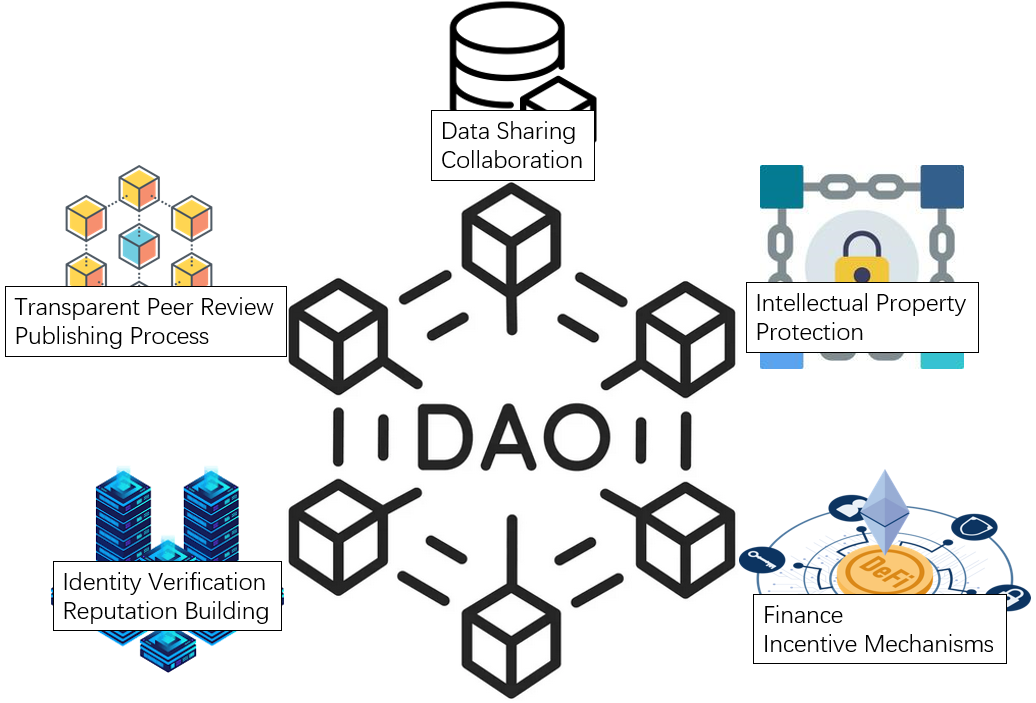
\includegraphics[width=\linewidth]{assets/dao.png}
  \caption{Application of DAO in Article and Journal}
  \label{fig:applicationofdao}
\end{figure}


According to the development of district DAO, related blockchain technology, the following DAO to Decentralized Scientific (DeSci) framework can be summarized as shown in the figure \ref{fig:applicationofdao}.It aims to establish a decentralized scientific publishing platform using blockchain and smart contract technology, enabling fair, transparent, and efficient scientific research dissemination \cite{wang2022dao}.
%按照区DAO,以及相关区块链技术的发展,可以如图总结出以下的DAO框架。它旨在通过区块链和智能合约技术,建立一个去中心化的科学出版平台,实现科学研究的公平、透明和高效。

\begin{itemize}
  \item \textbf{Transparent Peer Review and Publishing Process:} 
  
  Blockchain can be used to create a transparent academic publishing platform, ensuring transparency throughout the peer-review and publishing processes.\cite{nakamoto2008bitcoin} Smart contracts can manage review, publication, and payment procedures, ensuring traceability and fairness.
  %透明的学术出版: 区块链可以用于创建透明的学术出版平台,确保审稿和出版过程的透明性。智能合约可以管理审稿、出版和付款流程,确保可追溯和公平。

  \item \textbf{Protection of Intellectual Property:}
  
  Blockchain and smart contracts can safeguard authors' intellectual property, ensuring their works are not copied or distributed without permission \cite{gurkaynak2018intellectual}.
  %知识产权保护: 区块链和智能合约可用于保护作者的知识产权,确保其作品不会未经许可就被复制或传播。
  
  \item \textbf{Identity Verification and Reputation Building:} 
  
  Blockchain can be employed to establish scholars' identities and reputations \cite{radziwill2018blockchain}. Smart contracts can automate the validation of scholars' achievements, storing them on the blockchain.
  %身份验证和声誉建立: 区块链可用于建立学者的身份和声誉。智能合约可以自动化验证学者的成就,并将其存储在区块链上。
  
  \item \textbf{Data Sharing and Collaboration:} 
  
  Blockchain and smart contracts can facilitate data sharing and collaboration among scholars, ensuring data integrity and traceability \cite{praitheeshan2019security}.
  %数据共享和合作: 区块链和智能合约可用于促进学者之间的数据共享和合作,确保数据的完整性和来源可追溯。
  
  \item \textbf{Finance and Incentive Mechanisms:} 
  
  DAO and cryptocurrencies can be used to support research finance and incentive mechanisms.Funds can be allocated according to token weights \cite{schar2021decentralized}.
  %金融和激励机制: 区块链和加密货币可以用于支持学术研究的融资和激励机制。资金可以按照token为权重分配。
\end{itemize}

These application examples highlight the potential value of blockchain, smart contracts, and DAO technology in academic publishing and journal management. They enhance transparency, protect intellectual property, verify identity, automate processes, and encourage collaboration. As these technologies continue to evolve, they hold promise for further innovation and efficiency in academia \cite{vacca2021systematic}.
%这些应用示例突显了区块链、智能合约和DAO技术在学术出版和杂志管理方面的潜在应用,提高了透明度、知识产权保护、身份验证和自动化审稿流程。随着这些技术的不断发展,它们将有望为学术界提供更多的创新和效率。

\subsection{Web3-Based Journal DAO Framework}

\begin{figure*}[h!]
  \centering
  \subfloat[Database]{
    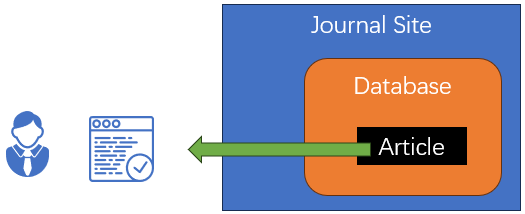
\includegraphics[width=2.4in]{assets/journalsite.png}
    \label{fig:database}
  }
  \hfil
  \subfloat[Blockchain]{
    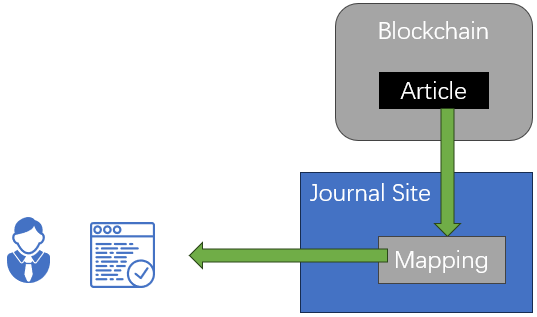
\includegraphics[width=3.6in]{assets/journalchain.png}
    \label{fig:blockchain}
    }
  \caption{Article in Database or Blockchain}
  \label{fig:storage}
\end{figure*}



In the traditional landscape of Web 2.0, the ownership of articles remains with the creators, yet the entirety of the associated data is ensconced within the databases of publishers, shrouded in a lack of transparency. This opaqueness extends to financial allocations, where, even if publishers express willingness to distribute funds, the absence of intermediary oversight poses challenges to ensuring fairness and accountability in the process. This paper delves into the transformative potential of Web 3.0 and blockchain technology within the DAO framework to rectify these issues, ushering in a new era of decentralized, transparent, and equitable financial distribution for content creators \cite{nath2014web}.
%在传统的Web 2.0领域,文章的所有权虽然归属于创作者,但所有相关数据都存储在由出版商的数据库中,缺乏透明度。即使出版商愿意分配资金,由于缺乏中介监管,这一过程也存在公正性和责任问题。本文深入探讨了Web 3.0和区块链技术在DAO框架内的转变潜力,以解决这些问题,引领创作者进入一个新时代,其中财务分配更为去中心化、透明和公平。
  


From a physical perspective, the data of articles is stored in the database of the journal website, as shown in Figure \ref{fig:database}. When regular users access the journal website, they can browse and download articles of interest. The interaction between users and the journal website typically involves the following steps.
When an article is uploaded to a blockchain, as shown in Figure \ref{fig:blockchain}, its content, timestamp, and relevant metadata are all recorded on the blockchain \cite{chowdhury2018blockchain}. This means that anyone can verify the existence, content, and timestamp of the article. This provides a high level of assurance for the immutability and transparency of documents, particularly with potential significance in research, intellectual property protection, and copyright. Uploading articles to the blockchain also enables decentralized data storage, reducing reliance on centralized institutions. This offers a more open and trustworthy means of data sharing for the academic community and other domains.Uploading an article to a blockchain, as compared to storing it in a traditional database, provides the author with a clear and objective ownership of the article. In a traditional database, the ownership of the data and the integrity of the database are controlled by the entity or organization managing the database. Authors and other stakeholders may not have direct control or visibility into the ownership and usage of the data.
%从物理层出发,期刊网站的数据库是文章数据的关键存储点。这些数据库通常位于服务器上,这些服务器可以分布在数据中心或云服务提供商的设施中。当普通用户访问期刊网站时,他们可以通过网络连接访问这些数据库以浏览和下载感兴趣的论文。
%%当一篇文章被上链到区块链中,它的内容、时间戳以及相关的元数据都会被记录在区块链上。这意味着任何人都可以验证这篇文章的存在、内容和时间。这为文献的不可篡改性和透明性提供了极高的保障,尤其在科研、知识产权保护和版权方面具有潜在的重要应用。上链文章还可以实现去中心化的数据存储,减少对中央化机构的依赖。这为学术界和其他领域提供了更开放和可信的数据共享方式。将文章上传至区块链,与将其存储在传统数据库中相比,可以让作者更明确且客观地拥有文章。在传统数据库中,数据的所有权和数据库的完整性由管理数据库的实体或组织控制。作者和其他利益相关方可能无法直接控制或了解数据的所有权和使用情况。

On the other hand, when an article is uploaded to a blockchain, the author can have greater confidence in their ownership and control over the article \cite{mcconaghy2017visibility}. The blockchain's decentralized and immutable nature ensures that the ownership records are transparent, tamper-resistant, and not under the sole control of a centralized authority. This empowers authors to have a direct and verifiable claim to their work, which can be particularly important for intellectual property protection, copyright, and ensuring that the author's rights are respected.
%另一方面,当文章上传至区块链时,作者可以更有信心地拥有和控制文章。区块链的去中心化和不可篡改性确保了所有权记录的透明性、防篡改性,并不受中心化权威的独立控制。这使作者能够直接并且可验证地主张他们的作品,这对于知识产权保护、版权以及确保作者的权利得到尊重尤为重要。



\subsection{Advantages of Finance in Journal DAO}


\begin{figure*}[!hb]
  \centering
  \subfloat[Web2.0]{
    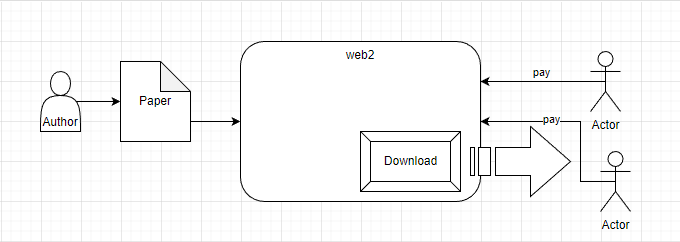
\includegraphics[width=3.2in]{assets/web2.png}
    \label{fig:payweb2}
  }
  \hfil
  \subfloat[Web3.0]{
    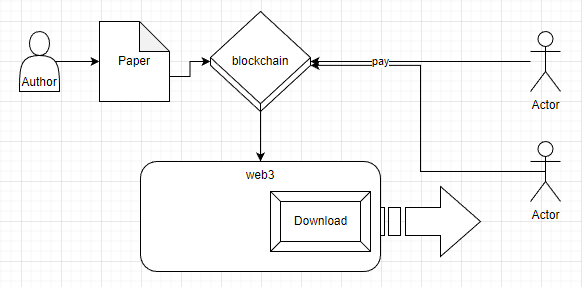
\includegraphics[width=3.2in]{assets/web3.png}
    \label{fig:payweb3}
  }
  \caption{Reader Pay for Download}
  \label{artcledownload}
\end{figure*}


In the evolution of electronic journals, websites have become the primary medium for disseminating research papers. Although the content of users' papers remains the intellectual property of the authors, the wealth generated by journals through these papers often belongs predominantly to the journals rather than the authors.In our hypothetical scenario, we contemplate a shift in this paradigm, envisioning a system where a certain proportion of the generated wealth is allocated back to the authors. Taking paid downloads as a simple example, this mechanism aims to provide authors with a more direct economic incentive. Such a transformation not only has the potential to enhance authors' motivation and creativity but also holds the promise of establishing a more equitable wealth distribution system. This envisioned change could contribute to fostering a sustainable and mutually beneficial development model in the realm of electronic journals, addressing the balance of interests between authors and journals more effectively.
% %在电子期刊的发展历程中,论文的载体逐渐从传统的印刷版本过渡到了数字化的网站形式。尽管用户的论文内容仍然属于作者的创作成果,然而,由于现行模式下,杂志通过论文创造的财富往往主要归属于杂志自身,而非作者。在当前设想下,我们可以假设一种改进模式,即按照一定比例将创造的财富回馈给作者。以付费下载为例,这一机制可以为作者提供更直接的经济回报。这种变革不仅有助于激发作者的积极性和创作动力,同时也有望促进更公正的财富分配体系的建立。这样的改变有望在电子期刊领域引入更加可持续和互惠的发展模式,从而更好地满足作者和杂志之间的利益平衡。


Web2, also known as the social web, refers to the current state of the internet that we use today, which is primarily focused on social media, e-commerce, and other web-based applications that allow users to interact with each other and with content in various ways. In Web2, payment systems are typically centralized, meaning that they are controlled by a single entity or organization. 
As the Figure \ref{fig:payweb2} shows. In the context of Web 2.0, the establishment of a platform for downloading articles entails several steps. Firstly, the creation of a functional website serves as the primary interface for users. This website acts as a centralized hub, hosting a database that stores a diverse range of articles across various disciplines.When a user decides to download a specific article, a payment system is in place to facilitate the transaction. The user pays a designated fee for the download, and the platform, acting as an intermediary, manages the distribution of funds. The allocation of funds may involve a proportional distribution to the authors, and this process is typically administered by the central entity running the website.This centralized model means that all user interactions, content storage, and payment transactions occur within the controlled environment of the website. Users depend on the centralized platform to oversee and coordinate all aspects of the transactional process, creating a reliance on a single authority for the entire operation \cite{yu2002electronic}.
%Web2,也称为社交网络,指的是我们今天使用的互联网的现状,主要集中在社交媒体、电子商务和其他基于网络的应用程序,这些应用程序允许用户相互交互以及与其他人进行交互。内容以多种方式呈现。在 Web2 中,支付系统通常是集中式的,这意味着它们由单个实体或组织控制。
%在Web 2.0的背景下,建立一个文章下载平台涉及到几个步骤。首先,创建一个功能齐全的网站作为用户的主要接口。这个网站充当了一个中心枢纽,托管一个数据库,存储了各个学科领域的多样化文章。当用户决定下载特定文章时,将会有一个支付系统来促成交易。用户支付一定费用进行下载,而平台则作为中介管理资金的分配。资金的分配可能涉及按比例分配给作者,这个过程通常由运营该网站的中央实体管理。这种中心化模式意味着所有用户交互、内容存储和支付交易都发生在网站的受控环境中。用户依赖于中心化平台监督和协调整个交易过程,因此对于整个操作都存在对单一权威的依赖。



Web3, also known as the decentralized web as shown in the Figure \ref{fig:payweb3}, represents a shift toward a more open, decentralized, and secure internet that is built on blockchain technology \cite{alabdulwahhab2018web}. In Web3, payment systems are decentralized, meaning that they are not controlled by a single entity or organization \cite{cao2022decentralized}. Instead, payments are made using cryptocurrency, which is a digital asset that is secured by cryptographic techniques and operates independently of central banks and other financial institutions. Cryptocurrency payments are processed directly between users without the need for intermediaries, which can result in lower transaction fees and faster processing times.
In the realm of Web 3.0, we witness a fundamental transformation in the dissemination of academic articles. Unlike the traditional Web 2.0 model, it introduces a paradigm shift. In this innovative framework, the data entity of articles resides directly on the blockchain, with the website serving as a mere interface reflecting the blockchain data. When users make payments for downloads, the entire fund allocation process is automated through smart contracts, eliminating the need for manual intervention. This groundbreaking framework ensures complete transparency and traceability throughout the process. As users pay to download articles, funds are automatically distributed according to the rules set within the DAO framework, without any centralized oversight.In the Web 3.0 paradigm, this novel model signifies a departure from reliance on traditional intermediaries. Instead, it empowers users with the direct participation in DAO frameworks, utilizing smart contracts for automated and secure fund distribution. This shift not only achieves decentralization in the transaction process but also enhances the efficiency of academic article transactions.In the Web 3.0 environment, articles are directly uploaded to the blockchain. All operations, including payment processing and fund distribution, are seamlessly executed through smart contracts. This innovative framework ensures complete transparency and traceability throughout the entire process. When users pay to download articles, the funds are automatically allocated according to the rules established within the DAO framework, eliminating the need for any centralized oversight.
%Web3,也称为去中心化网络,代表着向基于区块链技术构建的更加开放、去中心化和安全的互联网的转变。在 Web3 中,支付系统是去中心化的,这意味着它们不受单个实体或组织的控制。相反,支付是使用加密货币进行的,加密货币是一种由加密技术保护并独立于中央银行和其他金融机构运作的数字资产。加密货币支付直接在用户之间进行处理,无需中介机构,这可以降低交易费用并缩短处理时间。
%在Web 3.0的领域中,我们对待学术文章传播方式发生了根本性的变革。与传统的Web 2.0模式不同,它引入了一种新的框架。文章数据主体直接存在于区块链上,而网站仅仅是对区块链数据的映射。在这一新的框架下,用户支付下载后,整个资金分配的过程都通过智能合约进行自动化执行,无需手动干预。这一创新性框架确保了整个过程的完全透明性和可追溯性。当用户支付下载文章时,资金会根据去中心化自治组织(DAO)框架内设立的规则自动分配,无需任何集中监管。
%在Web 3.0的范式中,这一新兴模式标志着我们不再依赖传统中介机构。相反,它赋予用户直接参与DAO框架的权力,利用智能合约实现资金的自动化和安全分配。这一转变不仅实现了交易过程的去中心化,还提高了学术文章交易的效率。
%在Web 3.0的环境中,文章直接上链。所有操作,包括支付处理和资金分配,都通过智能合约无缝执行。这一创新性框架确保了整个过程的完全透明性和可追溯性。当用户支付下载文章时,资金会根据去中心化自治组织(DAO)框架内设立的规则自动分配,无需任何集中监管。



\subsection{The Operation Process of the Journal DAO}

In the practical implementation of the Journal DAO, this paper leveraged the Aragon framework to establish a decentralized and transparent infrastructure for academic publishing. The execution of the DAO involved several key steps to ensure a seamless and fair distribution of tokens among participants \cite{el2020overview}.
In a DAO, the concept of incentive mechanisms plays a crucial role in driving active participation and contributions. These mechanisms are designed to provide incentives and rewards to individuals or entities involved in the DAO's activities. By offering tangible benefits such as token rewards, governance rights, or recognition, participants are motivated to actively engage and contribute to the DAO's growth and development. Effective incentive mechanisms foster collaboration, maintain long-term motivation, and encourage innovation within the DAO community. The incentive design of journal dao promotes collaboration, maintains long-term incentives, and promotes innovation within the DAO community in the following aspects.
%在期刊 DAO 的实际实施中,我们利用 Aragon 框架建立了一个去中心化和透明的学术出版基础设施。 DAO 的执行涉及几个关键步骤,以确保代币在参与者之间的无缝和公正分配。
%在 DAO 中,激励机制的概念在推动积极参与和贡献方面发挥着至关重要的作用。这些机制旨在为参与 DAO 活动的个人或实体提供激励和奖励。通过提供代币奖励、治理权或认可等有形利益,参与者会被激励积极参与 DAO 的成长和发展并为其做出贡献。journal dao的激励设计在以下几个方面促进了协作、维护长期激励和促进DAO社区内的创新。

\begin{enumerate}
  \item Author Rewards:
  %作者奖励:

  Authors receive tokens based on the evaluation provided by reviewers during the submission process. The more constructive and impactful the reviews, the higher the token allocation to the authors.
  %作者根据评审人在提交过程中提供的评估获得代币。评审越有建设性和有影响力,作者获得的代币就越多。

  \item Reviewer Incentives:
  %评审者激励:
  
  Reviewers are rewarded with tokens for their valuable contribution to the peer-review process. This includes providing insightful feedback and assisting in maintaining the quality of published work.
  %评审者因其对同行评审过程的宝贵贡献而获得代币。这包括提供有深度的反馈和帮助维护已发布作品的质量。
  
  \item Publication and Download Rewards:
  %出版和下载奖励:
  
  Upon successful publication, both authors and users who download the papers are granted tokens. This encourages not only the creation of quality content but also its dissemination and accessibility.
  %在成功发布后,作者和下载论文的用户都会获得代币。这不仅鼓励了高质量内容的创作,还促进了其传播和获取。

  \item Citation Bonuses:
  %引用奖金:

  Authors receive additional tokens when their published work is cited by other researchers. This incentivizes the production of influential and impactful research that contributes to the academic community.
  %当其他研究人员引用作者已发布的作品时,作者将额外获得代币。这鼓励了产生有影响力和影响力研究的创作。

\end{enumerate}

\begin{figure}[h]
  \centering
  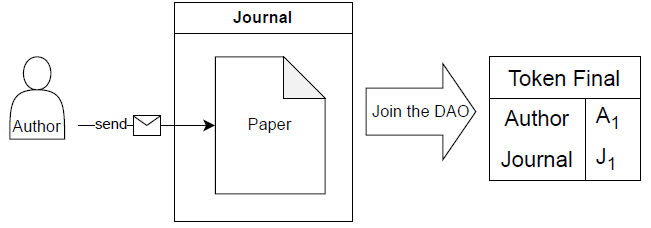
\includegraphics[width=3.2in]{assets/daopaper.png}
  \caption{Distribute Token by DAO}
  \label{fig:distributetoken}
\end{figure}


As Figure \ref{fig:distributetoken} shows, the process initiates with a user submitting a paper for publication. As the DAO initiates the coin minting process, specific rules govern the allocation of tokens. Authors are categorized based on their roles in the paper, including corresponding authors, first authors, second authors, and third authors, and so on, each receiving distinct token allocations.Simultaneously, reviewers play a pivotal role in the distribution of tokens. Their allocations are determined by their roles in the review process and the scores they assign to the submitted papers. This meticulous token distribution mechanism ensures that each contributor, whether an author or reviewer, is fairly rewarded according to their specific contributions and responsibilities.By implementing such a structured system, the DAO creates a transparent and equitable environment, aligning the incentives of authors and reviewers. This not only fosters a sense of fairness within the system but also encourages active and meaningful participation from all contributors. The workflow, guided by DAO principles, facilitates a seamless integration of various stakeholders, ensuring a well-functioning and self-sustaining ecosystem.
%在图示的工作流程中,流程始于用户提交论文进行出版。随着DAO启动铸币过程,特定规则指导着代币的分配。作者根据其在论文中的角色分为通讯作者、第一作者、第二作者和第三作者,每个人都获得不同的代币分配。同时,审稿人在代币分配中发挥着至关重要的作用。他们的分配由他们在审稿过程中的角色和对提交的论文的评分决定。这种细致入微的代币分配机制确保了每个贡献者,无论是作者还是审稿人,都能根据其具体的贡献和责任公正获得奖励。通过实施这样一个结构化的系统,DAO创造了一个透明而公平的环境,使作者和审稿人的激励保持一致。这不仅在系统内部培养了公正感,还鼓励各方积极而有意义地参与。受DAO原则指导的工作流程促进了各利益相关方的无缝整合,确保了一个运行良好且自我维持的生态系统。

\begin{figure}[h]
  \centering
  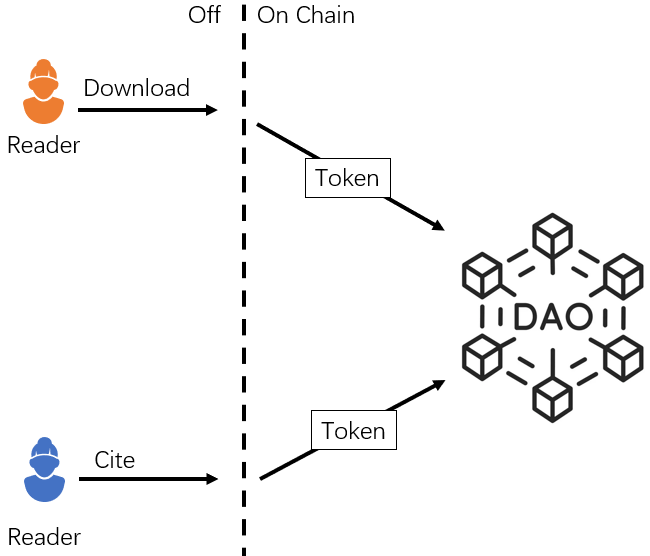
\includegraphics[width=3.2in]{assets/addtoken.png}
  \caption{Distribute Token while Download or cited}
  \label{fig:addtoken}
\end{figure}

As Figure \ref{fig:addtoken} shows, upon the download or citation of a paper, the DAO employs specific rules for the allocation of tokens to the downloader and the citers. This ensures that contributors beyond the authorship and reviewing process are also recognized and rewarded within the DAO framework.For downloaders, the token allocation is determined by the extent and impact of their engagement with the paper. High download counts result in increased token rewards, creating a dynamic and merit-based incentive system.Similarly, when a paper is cited, the citers receive token allocations based on the significance and reach of their citations. This encourages users to engage in scholarly discussions, contribute to the academic community, and actively participate in the dissemination of knowledge.These token allocation mechanisms not only acknowledge the efforts of those who contribute by downloading or citing papers but also foster a collaborative environment where users are motivated to interact with the content and contribute meaningfully to the scholarly ecosystem \cite{9994617}. The DAO's commitment to recognizing various forms of contribution ensures a comprehensive and inclusive reward system, aligning incentives with the broader goals of the academic community.
%在论文被下载或引用时,DAO会根据一定的规则给予下载者和引用者的token分配。这确保了在DAO框架内,除了作者和审稿过程之外的贡献者也能够得到认可和奖励。对于下载者,token的分配取决于他们与论文的互动程度和影响力。高下载次数会导致更多的token奖励,形成了一个动态且基于贡献的激励体系。同样,当论文被引用时,引用者将根据其引用的重要性和影响力获得token分配。这鼓励用户参与学术讨论,为学术界做出贡献,并积极参与知识的传播。这些token分配机制不仅承认了那些通过下载或引用论文做出贡献的人的努力,还促进了一个协作的环境,激励用户与内容互动,并有意义地为学术生态系统做出贡献。DAO对于认可各种形式贡献的承诺确保了一个全面而包容性的奖励体系,将激励机制与学术界更广泛的目标保持一致。


Non-Fungible Tokens (NFTs) are a type of digital asset that represent ownership or proof of authenticity of a unique item or piece of content on the blockchain \cite{wang2021non}. Unlike cryptocurrencies like Bitcoin or Ethereum, which are fungible and can be exchanged for one another, NFTs are unique and cannot be exchanged on a one-to-one basis.
The finance generated within the Journal DAO is distributed based on the NFT model, where each token holder is entitled to a proportional share. This innovative approach ensures that the financial rewards align with the level of contribution and engagement at various stages of the academic process \cite{nadini2021mapping}.
%不可替代代币(NFT)是一种数字资产,代表区块链上独特项目或内容的所有权或真实性证明。与比特币或以太坊等可替代且可以相互交换的加密货币不同,NFT 是独一无二的,不能一对一地进行交换。
%期刊 DAO 内生成的财务基于 NFT 模型进行分配,其中每个代币持有者有权获得相应份额。这种创新方法确保了财务奖励与在学术流程的各个阶段的贡献和参与程度相一致。


\begin{figure}[h]
  \centering
  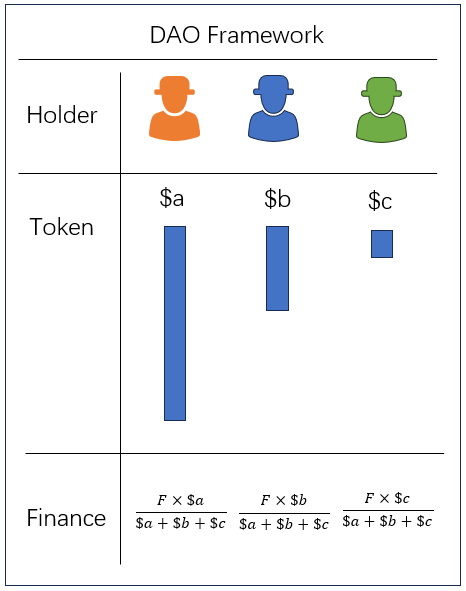
\includegraphics[width=3.2in]{assets/finance.png}
  \caption{Distribute Finance by NFTs}
  \label{fig:financenft}
\end{figure}

As Figure \ref{fig:financenft} shows, in this system, authors, reviewers, download users, and reference users all possess a specific quantity of tokens. These tokens are considered as NFTs due to their unique nature. Once finance is generated, such as when a user pays to download a paper, the system allocates this finance based on the number of tokens held by the respective parties.This design ensures objectivity, fairness, and transparency within the system. Each participant's contribution is reflected in a specific number of tokens, and the allocation mechanism operates according to the quantity of these tokens. Such a design not only enhances the fairness of the incentive mechanism but also makes the entire system more transparent, allowing participants to clearly understand the relationship between their contributions and rewards.This NFT-based token system provides tangible and verifiable returns for contributors while establishing an effective and operable incentive mechanism for the entire ecosystem \cite{kong2021alternative}. This fair and transparent allocation method is expected to drive collaboration and development in the academic community, creating a mutually beneficial environment for all stakeholders.

%在这个系统中,作者、审稿人、下载用户和引用用户都拥有一定数量的token。这些token具有唯一性,可以被视为NFT(非同质化代币)。一旦产生了finance,比如用户通过付费下载论文,系统会按照持有者的token数量来分配这部分finance。这个设计确保了系统的客观性、公正性和透明性。每个参与者的贡献都以特定数量的token体现,而分配机制则按照这些token的数量来进行。这样的设计不仅提高了激励机制的公正性,也使得整个系统更加透明,参与者可以清晰地了解他们的贡献与奖励之间的关系。这种以NFT为基础的token系统为贡献者提供了具体的、可证明的回报,同时也为整个生态系统提供了一种有效的、可操作的激励机制。这种公正而透明的分配方式有望推动学术界的合作与发展,为各方创造一个共赢的环境。




\subsection{Summary of Journal DAO}




Overall, the main difference in payment systems between Web2 and Web3 is the degree of centralization. Web2 payment systems are centralized, while Web3 payment systems are decentralized. While Web3 is still in its early stages, it has the potential to revolutionize the way we think about payments, transactions, and financial systems.
In the current era of digitization, the act of anchoring a paper on the blockchain signifies the author's complete ownership of the work, opening up boundless possibilities. The introduction of blockchain technology empowers authors with more rights and limitless potential. Once a paper is inscribed on the immutable blockchain, authors not only possess intellectual property rights but also gain absolute control over their creations. This shift in ownership implies that authors can explore innovation more freely, facilitate transparent data sharing, and attain fairer returns from the wealth generated by their works \cite{wang2023decentralized}. The immutability and transparency afforded by blockchain provide robust protection for the rights of paper owners, ushering in new possibilities for academic research and knowledge sharing. This profound ownership transformation elevates a paper beyond being merely a conduit for academic dissemination; it becomes a symbol of the unique wealth created by the author, sparking a profound revolution in the relationship between academia and authors.
%总体而言,Web2和Web3支付系统的主要区别在于中心化程度。 Web2支付系统是中心化的,而Web3支付系统是去中心化的。虽然 Web3 仍处于早期阶段,但它有潜力彻底改变我们对支付、交易和金融系统的看法。
%在这个时代,随着论文数字化的趋势,将论文上链意味着作者对其作品的彻底拥有。区块链技术的引入赋予了作者更多的权利和无限的可能性。一旦论文被写入不可篡改的区块链,作者不仅仅拥有了知识产权,更获得了对其作品的完全掌控。这样的所有权转变意味着作者可以更自由地探索创新、实现数据的透明共享,并在作品创造的财富中获得更为公平的回报。通过区块链的不可篡改性和透明性,论文的所有者权益得到了更强有力的保障,为学术研究和知识共享带来了新的可能性。这种彻底的拥有使得论文不再仅仅是学术传播的载体,更是作者创造的独特财富的象征,为学术界和作者之间的关系带来了深刻的变革。




  
\section{Mechanism Design of Journal DAO \label{sec:mechanism}}
% 这部分建议给一些符号和公式,如投稿时怎么分token,审稿时token怎么流转,下载和引用时token和finance怎么变化,这些都用公式描述出来

%把dao应用在journal。

%把dao应用在journal。作者,审稿人,读者都能受益。作者作为文章的拥有者,占有最多的最多的收益,并且随着时间的推移,收益会越来越高。审稿人作为文章的负责人,前期占有较高的收益,后期逐渐降低。读者作为文章的参与者,收益相对较低,但是越早参与,收益就越高。


% 本文结合DAO的基本概念,创建DAO的框架。首先是铸币,其中为所有与论文相关的参与者,包括审稿人,作者,读者,按照一定的机制分配token。token可以用来决定proposal的权重,本框架根据token分配finance。
This paper combines the fundamental concepts of DAO to establish a framework for implementing DAO in academic journals. The framework begins with the issuance of tokens, which are allocated to all participants involved in the publication process, including reviewers, authors, and readers, through a specified mechanism. These tokens serve as a means to determine the weightage of proposals, and the framework utilizes the token distribution to allocate financial resources accordingly. By integrating token-based incentives and governance mechanisms, this framework ensures a fair and transparent distribution of resources within the DAO-operated journal ecosystem. Participants holding tokens can actively participate in the processes of all aspects of the article publication, such as send articles, review articles, and download articles, thereby influencing the allocation of financial resources based on their token holdings. Through this framework, the DAO-operated journal can foster an inclusive and democratic environment, empowering participants to shape the direction and priorities of the journal based on their token weightage.
%本文结合DAO的基本概念,创建了一个适用于学术期刊的DAO框架。该框架首先进行铸币操作,将与论文相关的所有参与者(包括审稿人、作者和读者)按照一定的机制分配代币。这些代币可以用来决定提案的权重,本框架则根据代币分配财务资源。通过整合代币激励和治理机制,该框架确保在DAO运营的学术期刊生态系统中资源的公平和透明分配。持有代币的参与者可以积极参与文章发布过程,例如发布文章、审阅文章和下载文章,从而根据其代币持有量影响财务资源的分配。通过该框架,DAO运营的学术期刊能够营造一个包容和民主的环境,赋予参与者根据其代币权重来塑造期刊的方向和优先事项的权力。


\begin{equation}
  \begin{bmatrix}
    A_t \\
    E_t \\
    P_t \\
    R_t 
  \end{bmatrix}
  = 
  \omega_{t-1}
  \begin{bmatrix}
    A_{t-1} \\
    E_{t-1} \\
    P_{t-1} \\
    R_{t-1}
  \end{bmatrix}
  +
  \omega_{t-2}
  \begin{bmatrix}
    A_{t-2} \\
    E_{t-2} \\
    p_{t-2} \\
    R_{t-2}
  \end{bmatrix}
  +
  \cdot
  + 
  \omega_n
  \begin{bmatrix}
    A_n \\
    E_n \\
    P_n \\
    R_n
  \end{bmatrix}
  \label{eq:dao}
\end{equation}



By applying the DAO framework to academic journals in accordance with the proposed Equation \ref{eq:dao}, each action taken within the system has the potential to alter future benefits. Through a well-structured incentive mechanism, the entire DAO ecosystem can achieve a state of perfect autonomy. This means that the actions and decisions made by participants, including authors, reviewers, and readers, have a direct impact on the overall functioning and success of the journal. With the right incentives in place, the DAO-operated journal can foster a self-sustaining and self-regulating environment, where participants are motivated to actively engage, contribute their expertise, and collectively drive the advancement of scholarly knowledge.
% 通过根据提议的方程 \ref{eq:dao} 将 DAO 框架应用于学术期刊,系统内采取的每项行动都有可能改变未来的效益。通过结构良好的激励机制,整个DAO生态系统可以达到完美自治的状态。这意味着包括作者、审稿人和读者在内的参与者的行动和决定对期刊的整体运作和成功有直接影响。通过适当的激励措施,DAO 运营的期刊可以营造一个自我维持和自我调节的环境,激励参与者积极参与、贡献他们的专业知识,并共同推动学术知识的进步。


\subsection{First Mint Token}

In the DAO framework, tokens are minted during key events such as article publication, downloads, and citations, and then distributed to participants according to predetermined proportions. All these processes are executed through smart contracts, ensuring transparency and traceability. Having a well-designed token allocation mechanism forms the foundation of the entire framework, enabling a self-sustaining and self-regulating environment.
With a fair token distribution mechanism, the DAO framework can create a system where participants are incentivized to contribute and engage actively. The allocation of tokens based on specific events fosters a sense of fairness and encourages collaboration among authors, readers, reviewers, and publishers. The transparent and traceable nature of the smart contract-based processes ensures that the token distribution is open to scrutiny and can be verified by all participants.
In this self-regulating environment, the DAO framework can adapt and adjust dynamically based on the actions and contributions of its participants. The token allocation mechanism serves as a means to reward and recognize the efforts of contributors, fostering a sustainable ecosystem where knowledge sharing and collaboration thrive.
% DAO框架在关键的事件进行铸币,如文章的发布,被下载,被引用,然后按照一定比例将其分发给各个参与者。所有过程经过智能合约完成,保证透明以及可追溯。有了合理的token分配机制,是整个框架的基础,可以实现自我维护和自我调节的环境。

\begin{equation}
  \begin{aligned}
    D_0 &= \sum_{i = 1}^{m}x_i \\
    1 &= \alpha_1 + \alpha_2 + \alpha_3 \\
    A_0 &= \alpha_1 D_0 \quad (A=\{a_0, a_1, a_2, a_3, \cdots a_n\}) \\
    E_0 &= \alpha_2 D_0 \quad (E=\{e_1, e_2, e_3, \cdots e_m\}) \\
    P_0 &= \alpha_3 D_0 \quad (P=\{p\})
  \end{aligned}
  \label{eq:dao0}
\end{equation}

Upon publication of an article, a DAO specific to that particular article is established, and tokens are minted and distributed among the authors, reviewers, and the publisher. The total number of tokens minted after this process, denoted as $D_0$, is determined based on Equation \ref{eq:dao0}, taking into account the distribution proportions among the three parties: $\alpha_1$, $\alpha_2$, and $\alpha_3$. Consequently, the allocation of tokens is as follows: the authors receive $A_0 = \alpha_1 D_0$, the reviewers receive $E_0 = \alpha_2 D_0$, and the publisher receives $P_0 = \alpha_3 D_0$.
%文章发表时候,创建一个当前article的DAO,铸币分给作者,审稿人和出版商。根据公式\ref{eq:dao0}$D_0$为本次铸币之后的总token数量,三方占比为$\alpha_1$,$\alpha_2$和$\alpha_3$。则作者分到$A_0 = \alpha_1 D_0 $,审稿人分到$E_0 = \alpha_2 D_0 $,出版商分到$P_0 = \alpha_3 D_0 $


\begin{equation}
  \begin{aligned}
    1 &= \beta_0 + \beta_1 + \beta_2 + \beta_3 + \cdots + \beta_n (\beta_1 \geq  \beta_2 \geq \beta_3 \cdots \geq \beta_n)\\
    a_{i} &= \beta_i A \quad (a \in A) \\
    a_{i0} &= \beta_i A_0 \quad (a_0 \in A_0 )
  \end{aligned}
  \label{eq:authorrate}
\end{equation}

In the case of having a total of $n$ authors, the allocation of tokens for each author is determined by the proportions specified in Equation \ref{eq:authorrate}. In this equation, $\beta_0$ represents the token allocation for the corresponding author, $\beta_1$ represents the token allocation for the first author, $\beta_2$ represents the token allocation for the second author, and so on. The total number of tokens allocated to all authors is denoted as $A$, and each author $a_i$ receives a portion of tokens distributed according to the respective $\beta$ ratio.When the article is published, tokens are minted and distributed to all authors. The total number of tokens allocated to the authors is denoted as $A_0$, and each author $a_{i0}$ receives tokens distributed in the same proportions as determined by the $\beta$ ratios.
%作者数量为n,每个作者分到的的token数量占比见公式\ref{eq:authorrate},其中$\beta_0$特指为通讯作者,$\beta_1$为一作,$\beta_2$为二作,以此类推。所有作者的token为$A$,每个作者$a_i$的token按照$\beta$比例分配。文章法布时,铸币给所有作者的token数量为$A_0$,每个作者$a_i0$按照同样的比例分配。

\begin{equation}
  \begin{aligned}
    1 &= \gamma_1 + \gamma_2 + \gamma_3 + \cdots + \gamma_m \\
    e_{i} &= \gamma_i E \quad (e \in E) \\
    e_{i0} &= \gamma_i E_0 \quad (e_0 \in E_0 )
  \end{aligned}
  \label{eq:reviewerrate}
\end{equation}

The number of reviewers is denoted as $m$, the allocation of tokens for each reviewer follows the proportions specified in Equation \ref{eq:reviewerrate}. In this equation, the token allocation for each reviewer $e_i$ is determined by the respective $\gamma$ ratio. The proportions for the reviewers may be determined based on other factors, such as the role the reviewers. The total number of tokens allocated to all reviewers is denoted as $E$.When the article is published, tokens are minted and distributed to all reviewers. The total number of tokens allocated to the reviewers is denoted as $E_0$, and each reviewer $e_{i0}$ receives tokens distributed in the same proportions as determined by the $\gamma$ ratios. The distribution mechanism remains consistent with that of the authors.
%审稿人数量为m,每个审稿审稿人分到的token数量占比见公式\ref{eq:reviewerrate},审稿人分得的比例按照其他方式决定,如角色定位。与作者相同,所有审稿人的token为$E$,每个审稿人$e_i$的token按照$\gamma$比例分配。文章法布时的铸币分配方式与之前相同,所有审稿人的token数量为$E_0$,每个审稿人$e_i0$按照$\gamma$比例分配。

\subsection{Token Distributement while User Download or Cite Article}


\begin{equation}
  \begin{aligned}
    D_1 &= D_{1a} + D_{1r} \\
    A_1 &= D_{1a} \\
    \Sigma^A_1 &= A_0 + A_1 \\
    E_1 &= 0 \\
    P_1 &= 0 \\
    R_1 &= D_{1r} \\
  \end{aligned}
  \label{eq:downloadtoken}
\end{equation}

After the publication of the article, when users read and download the article, additional token minting occurs according to the formula specified in Equation \ref{eq:downloadtoken}. The purpose of this additional token minting is to incentivize authors and provide benefits to readers. In this process, new tokens are allocated to both authors and readers, while the token allocations for reviewers and the publisher remain unchanged.
% 文章法布之后,有用户阅读并下载了文章,此时会继续铸币,见公式\ref{eq:downloadtoken}。为了鼓励作者,以及让利给读者,新的token分给作者以及读者,审稿人以及出版商的token保持不变。

\begin{equation}
  \begin{aligned}
    1 &= \beta_{1, 0} + \beta_{1, 1} + \beta_{1, 2} \\
    a_{1,0} &= A_1 \beta_{1, 0}  \\
    a_{1,1} &= A_1 \beta_{1, 1}  \\
    a_{1,2} &= A_1 \beta_{1, 2}  \\
  \end{aligned}
  \label{eq:downloadrate}
\end{equation}

According to Equation \ref{eq:downloadrate}, the tokens generated through the user's download behavior will be allocated to the corresponding author, first author, and second author in certain proportions. However, the token allocations for other authors remain unchanged.
% 根据公式\ref{eq:downloadrate},用户下载行为时铸币生成的token,会按照一定的比例分给通讯作者,一作以及二作,其他作者的token保持不变。


\begin{equation}
  \begin{aligned}
    D_2 &= D_{2a} + D_{2r} \\
    A_2 &= D_{2a} \\
    \Sigma^A_2 &= A_0 + A_1 + A_2 \\
    E_2 &= 0 \\
    P_2 &= 0 \\
    R_2 &= D_{2r} \\
    \Sigma_{r1} & = R_1 + R_2 \quad if \quad R_1 = R_2 \quad (r_1 \in R ) 
  \end{aligned}
  \label{eq:citetoken}
\end{equation}

According to Equation \ref{eq:citetoken}, if a user cites a previously downloaded article in their own article, it triggers token minting. The tokens generated in this case are allocated to both the authors of the cited article and the user who made the citation.
% 根据公式\ref{eq:citetoken},用户自己发了论文引用了之前下载的论文,也会出发铸币,token同样分给作者以及引用的用户。



\subsection{Finance by Token}

By employing token allocation based on NFT principles, the framework ensures a fair distribution of rewards among token holders. Through transparent smart contracts, the DAO framework establishes a self-regulating environment that incentivizes active participation and contribution. The implementation of this token-based distribution mechanism requires tracking token ownership and automated distribution of finance.
% 按照nft的方式,把token作为分配的比例,一旦产生了finance,就按照所有holder都可以按照比分到finance。

\begin{equation}
  \begin{aligned}
    1 &= \frac{A}{D} + \frac{E}{D} + \frac{P}{D} + \frac{R}{D} = \alpha_1 + \alpha_2 + \alpha_3 + \alpha_4 \\
    F &= finance \\
    F_A &= \alpha_1 F \quad (A=\{a_0, a_1, a_2, a_3, \cdots a_n\}) \\
    F_E &= \alpha_2 F \quad (E=\{e_1, e_2, e_3, \cdots e_m\}) \\
    F_P &= \alpha_3 F \quad (P=\{p\}) \\ 
    F_R &= \alpha_4 F \quad (R=\{r_1, r_2, r_3, \cdots r_i\})
  \end{aligned}
  \label{eq:finance}
\end{equation}


According to Equation \ref{eq:finance}, the token allocation ratios for authors, reviewers, publisher, and readers are denoted as $\alpha_1$, $\alpha_2$, $\alpha_3$, and $\alpha_4$, respectively. Once finance is generated, it is distributed to all token holders based on these ratios. 
To respect intellectual property rights, many publishers require users to pay for downloading articles. In such cases, finance enters the DAO and is distributed to all authors, reviewers, publisher, and readers according to their token ratios. Articles typically attract a significant number of downloads, with exceptional ones garnering even more. Importantly, this distribution mechanism enables sustained earnings, thereby incentivizing authors to produce higher quality articles. 
While users initially act as consumers when downloading articles, they also become partial owners of the downloaded articles. As a result, they are eligible to receive a portion of the generated finance based on their token ratios. Motivating readers is crucial as it encourages them to willingly pay for article downloads, ultimately creating more finance and fostering a real automated organization. 
By implementing this approach, all participants receive fair allocations for their contributions. The autonomous nature of the framework drives authors to produce outstanding articles and incentivizes readers to pay for downloads, thereby generating more finance and establishing a virtuous cycle within the system.
% 根据公式\ref{eq:finance},作者、审稿人、出版商、读者的token分配比例为$\alpha_1$, $\alpha_2$, $\alpha_3$, $\alpha_4$,一旦产生finance,会按照这个比例分给所有holder。比如为了尊重知识产权,很多出版商的论文需要用户付费下载,此时就有了finance进入DAO,并按照token的比例分给了所有作者、审稿人、出版商、读者。文章的下载量一般会很多,优秀的文章下载量更多,最重要的是可以持续收益,这种情况下,激励了作者写出更优秀的article。用户作为读者下载文章本是消费者,但是下载文章之后既变成文章的拥有者之一,之后的finance也会分给这个读者。对读者的激励十分重要,这让读者更愿意付费下载article,也就创造了更多的finance,形成一个完美的自治。

\begin{figure}[h]
  \centering
  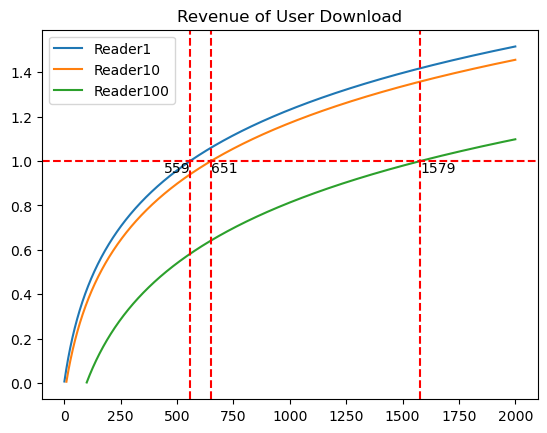
\includegraphics[width=3.2in]{assets/revenue-user-download.png}
  \caption{Revenue of User Download.}
  \label{fig:revenue-user-download}
\end{figure}

The total revenue for downloading users is depicted in Figure \ref{fig:revenue-user-download}. As readers who own the downloaded articles, their total revenue increases with a growing number of users downloading the articles. However, as more readers download the article and become owners, the individual token proportion naturally decreases. Consequently, the per-download revenue gradually declines.
To simulate the distribution ratios, let's consider the following scenario: the first reader who downloads the article breaks even when the article is downloaded 559 times; the tenth reader breaks even when the article reaches 651 downloads; and the one hundredth reader breaks even at a staggering 1579 downloads. This incentive mechanism aims to encourage readers to discover exceptional articles earlier rather than following the crowd since owning the article no longer yields significant returns.
This approach incentivizes readers to identify outstanding articles sooner, as the potential for substantial earnings diminishes once an article has already demonstrated its quality.
% 下载用户的总收益如图 \ref{fig:revenue-user-download} 所示,随着更多用户下载article,作为读者的article拥有者,总收益会越来越多,但是因为更多其他读者下载article也获取了token,成为了article的拥有者,自己token的占比势必会减少,所以单次收益逐渐降低。设定分配比例进行模拟,第一个下载论文的读者,在文章被下载559次时,总收入与下载时的支出持平;第十个下载论文的读者,收支相抵时候需要文章被下载651次;第一百个下载论文的读者,收支相抵更是要到1579次。此种激励方式在于,如果文章已经证明很优秀了,再拥有已经不能得到多少收益了,鼓励读者更早发现优秀的文章,而不是跟风。


\begin{figure}[h]
  \centering
  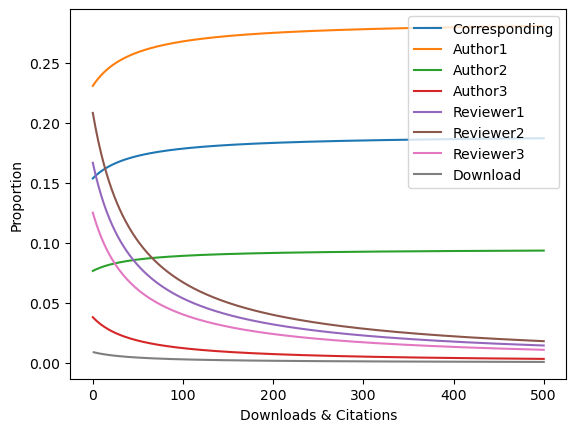
\includegraphics[width=3.2in]{assets/proportion-all.png}
  \caption{Proportion of All.}
  \label{fig:proportion-all}
\end{figure}

Integrating DAO technology into the realm of academic journals holds immense potential for benefiting authors, reviewers, and readers alike. Look at Figure \ref{fig:proportion-all}.
Authors, being the rightful owners of their published works, would reap the most substantial rewards from such a system. By leveraging the decentralized nature of DAOs, authors can secure a greater share of the financial gains associated with their articles. As time progresses, their earnings could potentially increase, providing a long-term incentive for continued contributions.
Reviewers, as the gatekeepers and custodians of scholarly integrity, would also stand to gain from the implementation of DAOs in journals. Initially, they would hold a higher proportion of benefits, reflecting their crucial role in the early stages of article evaluation. However, as time progresses and articles are published, their share of benefits may gradually diminish, ensuring a fair distribution of rewards among all stakeholders.
Readers, as active participants in the scholarly discourse, would also have the opportunity to benefit from DAO-operated journals. While their gains may be comparatively lower than authors and reviewers, early engagement with the DAO ecosystem could yield higher returns. By accessing articles and participating in the DAO's governance processes, readers can contribute to the growth and success of the journal, potentially increasing their benefits over time.
The implementation of DAO mechanisms, such as token-based incentives, transparent governance structures, and decentralized decision-making processes, would enable a fair and equitable model for academic journals. This model fosters a sense of ownership, rewards active participation, and ensures the sustainability and long-term viability of the journal ecosystem.
%将 DAO 技术整合到学术期刊领域具有巨大的潜力,可以使作者、审稿人和读者受益
%作者作为其已发表作品的合法所有者,将从这样的系统中获得最丰厚的回报。通过利用 DAO 的去中心化性质,作者可以获得与其文章相关的更大份额的经济收益。随着时间的推移,他们的收入可能会增加,从而为持续贡献提供长期激励。
%审稿人作为学术诚信的看门人和守护者,也将从期刊中 DAO 的实施中获益。最初,他们将获得较高比例的收益,这反映了他们在文章评估的早期阶段的关键作用。然而,随着文章的发布,他们的利益份额可能会逐渐减少,从而确保所有利益相关者之间公平分配奖励。
%读者作为学术讨论的积极参与者,也将有机会从 DAO 运营的期刊中受益。虽然他们的收益可能相对低于作者和审稿人,但早期参与 DAO 生态系统可能会产生更高的回报。通过访问文章并参与 DAO 的治理流程,读者可以为期刊的发展和成功做出贡献,并有可能随着时间的推移增加其收益。
%DAO 机制的实施,例如基于代币的激励、透明的治理结构和去中心化的决策流程,将为学术期刊提供公平公正的模式。这种模式培养主人翁意识,奖励积极参与,并确保期刊生态系统的可持续性和长期生存能力。


\subsection{Decentralized Governance}
%去中心化治理:

DAO, adopting a decentralized governance model, allows token holders to participate in the decision-making process. This ensures community involvement in platform development, creating a democratic and inclusive environment. With robust incentives in place, token holders have made outstanding contributions while also receiving greater rewards. This positive feedback loop forms a self-sustaining ecosystem of active governance. DAOs leverage blockchain technology to provide transparency and trust, recording all proposals, votes, and transactions on the blockchain for public verification. Incentives motivate token holders to actively engage in the governance process, while DAOs offer a meritocratic approach that values expertise. The flexibility and adaptability of DAOs allow them to evolve and respond to the needs of the community. However, challenges such as active participation, governance gridlocks, and power concentration need to be addressed through clear rules and mechanisms. Overall, DAOs empower token holders, foster community involvement, and create a democratic and inclusive environment.
%DAO采用去中心化治理模型,允许代币持有者参与决策过程。这确保了社区能够参与平台发展,创造了一个民主和包容的环境。在比较优秀的激励下,代币持有者做了出色的贡献,同时也获得更多的奖励。一个积极的自治体系完美闭环。DAO借助区块链技术提供透明度和信任度,将所有提案、投票和交易记录在区块链上,供公众验证。激励机制激励代币持有者积极参与治理过程,而DAO则提供了重视专业知识的优秀人才的机会。DAO的灵活性和适应性使其能够随着社区的需求而发展和应对变化。然而,需要通过明确的规则和机制来解决积极参与、治理僵局和权力集中等挑战。总体而言,DAO赋予代币持有者权力,促进社区参与,并创造民主和包容的环境。

The implementation of the Journal DAO has yielded positive results in terms of increased engagement, quality submissions, and a more inclusive academic ecosystem. The transparent and automated token distribution mechanisms have effectively addressed issues of ownership and reward distribution, fostering a collaborative and fair scholarly environment.
In conclusion, The detailed execution of the Journal DAO demonstrates the viability of blockchain and DAO principles in reshaping academic publishing. The emphasis on decentralized governance, token incentives, and transparent finance distribution has the potential to revolutionize the scholarly landscape, making it more accessible, collaborative, and equitable for all participants.
%期刊 DAO 的实施在提高参与度、质量投稿以及创建更具包容性的学术生态方面取得了积极成果。透明和自动化的代币分配机制有效解决了所有权和奖励分配的问题,促进了合作和公正的学术环境。
%总的来说,期刊 DAO 的详细执行展示了区块链和 DAO 原则在重塑学术出版方面的可行性。对去中心化治理、代币激励和透明财务分配的强调有望彻底改变学术领域,使其对所有参与者更具可访问性、合作性和公平性。

\section{Model performance \label{sec:performance}}


\begin{table*}[ht!]
  \begin{center}
    \caption{Finance for DAO.}
    \label{tab:finance}
    \begin{tabular}{r|l|l|l|l|l|l|l|l|l} % <-- Alignments: 1st column left, 2nd middle and 3rd right, with vertical lines in between
      & \multicolumn{4}{c}{\textbf{Authors}} & \multicolumn{3}{|c|}{\textbf{Reviewers}} & \multicolumn{2}{c}{\textbf{Readers}}\\
      \hline
      \textbf{index} & \textbf{Corresponding} & \textbf{Author1} & \textbf{Author2} & \textbf{Author3} & \textbf{reviewer1} & \textbf{reviewer2} & \textbf{reviewer3} & \textbf{cite} & \textbf{download}\\
      \hline
      0 & 0.128171 & 0.128171 & 0.051068 & 0.025367 & 0.222296 & 0.278037 & 0.166889 & 0.000000 & 0.000000 \\
      1 & 0.128605 & 0.128605 & 0.051044 & 0.025191 & 0.220749 & 0.276102 & 0.165728 & 0.000000 & 0.003977 \\
      2 & 0.129032 & 0.129032 & 0.051020 & 0.025016 & 0.219223 & 0.274194 & 0.164582 & 0.000000 & 0.003950 \\
      3 & 0.129454 & 0.129454 & 0.050997 & 0.024845 & 0.217718 & 0.272311 & 0.163452 & 0.000000 & 0.003923 \\
      4 & 0.129870 & 0.129870 & 0.050974 & 0.024675 & 0.216234 & 0.270455 & 0.162338 & 0.000000 & 0.003896 \\
      5 & 0.130281 & 0.130281 & 0.050951 & 0.024508 & 0.214769 & 0.268623 & 0.161238 & 0.000000 & 0.003870 \\
      6 & 0.130685 & 0.130685 & 0.050929 & 0.024343 & 0.213325 & 0.266816 & 0.160154 & 0.000000 & 0.003844 \\
      7 & 0.130982 & 0.130982 & 0.050693 & 0.023929 & 0.209698 & 0.262280 & 0.157431 & 0.007557 & 0.003778 \\
      8 & 0.131373 & 0.131373 & 0.050673 & 0.023772 & 0.208320 & 0.260557 & 0.156397 & 0.007507 & 0.003754 \\
      9 & 0.131759 & 0.131759 & 0.050653 & 0.023617 & 0.206961 & 0.258856 & 0.155376 & 0.007458 & 0.003729 \\
      10 & 0.132140 & 0.132140 & 0.050633 & 0.023464 & 0.205619 & 0.257178 & 0.154369 & 0.007410 & 0.003705 \\
      11 & 0.132515 & 0.132515 & 0.050613 & 0.023313 & 0.204294 & 0.255521 & 0.153374 & 0.007362 & 0.003681 \\
      12 & 0.132886 & 0.132886 & 0.050594 & 0.023164 & 0.202987 & 0.253886 & 0.152393 & 0.007315 & 0.003657 \\
      13 & 0.133253 & 0.133253 & 0.050575 & 0.023016 & 0.201696 & 0.252271 & 0.151423 & 0.007268 & 0.003634 \\
      14 & 0.133614 & 0.133614 & 0.050557 & 0.022871 & 0.200421 & 0.250677 & 0.150466 & 0.007222 & 0.003611 \\
      15 & 0.133971 & 0.133971 & 0.050538 & 0.022727 & 0.199163 & 0.249103 & 0.149522 & 0.007177 & 0.003589 \\
      16 & 0.134324 & 0.134324 & 0.050520 & 0.022585 & 0.197920 & 0.247548 & 0.148588 & 0.007132 & 0.003566 \\
      17 & 0.134672 & 0.134672 & 0.050502 & 0.022445 & 0.196692 & 0.246013 & 0.147667 & 0.007088 & 0.003544 \\
      18 & 0.135016 & 0.135016 & 0.050484 & 0.022307 & 0.195480 & 0.244497 & 0.146757 & 0.007044 & 0.003522 \\
      19 & 0.135356 & 0.135356 & 0.050467 & 0.022170 & 0.194282 & 0.242999 & 0.145858 & 0.007001 & 0.003501 \\
      20 & 0.135692 & 0.135692 & 0.050449 & 0.022035 & 0.193099 & 0.241519 & 0.144970 & 0.006959 & 0.003479 \\
      Total & 2.773651 & 2.773651 & 1.064935 & 0.495363 & 4.340948 & 5.429444 & 3.258970 & 0.101500 & 0.074210 \\
    \end{tabular}
  \end{center}
\end{table*}

In addition to the theoretical framework, there need conducted simulations to evaluate the effectiveness of the proposed DAO system \cite{macal2009agent}. Table \ref{tab:finance} presents results from 20 simulated downloads, illustrating the distribution of finance among holders. This simulation provides a comprehensive overview of how finance is allocated to holders based on their token holdings.
Within the DAO framework, authors, as the owners of the articles, experience an increase in their tokens and ownership ratio when their articles are downloaded or cited, leading to higher profits. Reviewers, as participants in the article review process, initially receive tokens that do not increase over time. Although their ownership ratio gradually decreases, their profits continue to increase. The accuracy of their ratings directly benefits themselves. Readers, during the process of downloading and citing, also receive tokens, albeit in smaller quantities and with lower ownership ratios. However, as the articles are downloaded or cited, their overall profits increase. Additionally, the profit margin gradually decreases, meaning that readers who download and cite the articles in the early stages will benefit from higher profits, thus incentivizing the early identification of outstanding articles.
%在论文中,我们不仅提出了理论框架,还进行了模拟实验来评估提出的DAO系统的有效性。表格1展示了20次模拟下载的结果,说明了finance在持有者之间的分配情况。这个模拟提供了一个全面的概述,说明了根据令牌持有情况如何分配finance。
% 在这个dao框架之下,author作为文章的拥有者,在文章被下载或被引用时,其token会增加,并且占有率也在增加,同时收益就会越来越高。reviewer作为文章的参与者,他们初期会收到相应的token,但是不再增加,虽然占比逐渐降低,但是收益总是是增加的,评分越准,对自己越有利。reader在download以及cite过程中,都会收到相应的token,虽然量少,并且占有率也不高,但是随着文章被下载或被引用,总收益就也会越来越高。并且在这个过程中,收益率是逐渐下降的,也就是在论文早期下载和引用的reader,会活动比较高的收益,这鼓励了早期识别优秀的论文。

\begin{table*}[t!]
  \begin{center}
    \caption{Finance of Real Article for DAO.}
    \label{tab:realpaper}
    \begin{tabular}{r|l|l|l|l|l|l|l|l|l} % <-- Alignments: 1st column left, 2nd middle and 3rd right, with vertical lines in between
       & \multicolumn{4}{c}{\textbf{Authors}} & \multicolumn{3}{|c|}{\textbf{Reviewers}} & \multicolumn{2}{c}{\textbf{Readers}}\\
       \hline
      \textbf{index} & \textbf{Corresponding} & \textbf{Author1} & \textbf{Author2} & \textbf{Author3} & \textbf{reviewer1} & \textbf{reviewer2} & \textbf{reviewer3} & \textbf{cite} & \textbf{download}\\
      \hline
      0 & 0.128171 & 0.128171 & 0.051068 & 0.025367 & 0.222296 & 0.278037 & 0.166889 & 0.000000 & 0.000000 \\
      1 & 0.128605 & 0.128605 & 0.051044 & 0.025191 & 0.220749 & 0.276102 & 0.165728 & 0.000000 & 0.003977 \\
      2 & 0.129032 & 0.129032 & 0.051020 & 0.025016 & 0.219223 & 0.274194 & 0.164582 & 0.000000 & 0.003950 \\
      3 & 0.129454 & 0.129454 & 0.050997 & 0.024845 & 0.217718 & 0.272311 & 0.163452 & 0.000000 & 0.003923 \\
      4 & 0.129870 & 0.129870 & 0.050974 & 0.024675 & 0.216234 & 0.270455 & 0.162338 & 0.000000 & 0.003896 \\
      ... & ... & ... & ... & ... & ... & ... & ... & ... & ... \\
      2151 & 0.209045 & 0.209045 & 0.043698 & 0.001416 & 0.012405 & 0.015516 & 0.009313 & 0.000447 & 0.000224 \\
      2152 & 0.209049 & 0.209049 & 0.043698 & 0.001415 & 0.012400 & 0.015509 & 0.009309 & 0.000447 & 0.000223 \\
      2153 & 0.209052 & 0.209052 & 0.043698 & 0.001414 & 0.012395 & 0.015503 & 0.009305 & 0.000447 & 0.000223 \\
      2154 & 0.209056 & 0.209056 & 0.043697 & 0.001414 & 0.012389 & 0.015496 & 0.009301 & 0.000446 & 0.000223 \\
      Total & 423.722713 & 423.722713 & 96.973407 & 9.477511 & 83.052922 & 103.878504 & 62.352043 & 2.672524 & 1.492444 \\
    \end{tabular}
  \end{center}
\end{table*}

Furthermore, we applied our DAO framework to a real-world case by analyzing a published paper with 2154 downloads and 42 citations. As shown in Table \ref{tab:realpaper}. By simulating the income distribution within the current DAO structure, we observed that download users not only offset their initial payment but also gained additional earnings. The incentivized system encourages users to respect copyright and, more importantly, has achieved a level of autonomy.The provided tables and case study demonstrate the practical application and positive outcomes of our proposed DAO framework. By aligning incentives with user behaviors, the system not only offsets costs for downloaders but also significantly incentivizes engagement. This not only respects copyright but also establishes a self-sustainable and autonomous ecosystem, providing valuable insights for the future development of decentralized academic publishing.

%此外,我们将DAO框架应用于一个真实案例,分析了一篇被下载2154次、引用42次的论文。通过模拟当前DAO结构下的收入分配情况,我们观察到下载用户不仅抵消了初始支付,还获得了额外的收益。这个激励系统鼓励用户尊重版权,更重要的是实现了一定程度的自治。提供的表格和案例研究展示了我们提出的DAO框架的实际应用和积极成果。通过将激励与用户行为保持一致,该系统不仅为下载者抵消了成本,还极大地激励了用户参与。这不仅尊重版权,还建立了一个自我可持续和自治的生态系统,为分散的学术出版的未来发展提供了有价值的见解。



After voluntarily making a payment, users' ability to participate contributes to a robust incentive mechanism, fostering a sense of autonomy within the entire framework. Through this design, users become direct contributors to financial activities, injecting new value into the framework and creating potential opportunities for self-reward. This decentralized autonomous model empowers users to engage directly in decision-making and contributions, shaping a more open, fair, and virtuous ecosystem. Overall, this autonomous framework cultivates a more positive and sustainable participation experience for users and the entire community.
Through the detailed simulations and analyses, the incentive mechanisms within the DAO framework emerge as crucial drivers in shaping the dynamics of authorship and user participation. As downloads and citations increase, the token-driven rewards become a powerful motivator for authors, leading to an accumulation of influence and financial gains. This incentive structure not only acknowledges and rewards the contributions of authors but also establishes a direct correlation between their efforts and the benefits they accrue.
Furthermore, users who engage with the system by downloading papers witness a direct impact on their influence and, subsequently, on their earnings. This creates a dual incentive structure, where authors and users are mutually motivated to contribute to and participate in the DAO environment. The concept of decentralized autonomy becomes evident as the system operates independently, fostering a self-sustaining loop of contributions, rewards, and governance.
In this context, the DAO framework provides a powerful tool for aligning interests and promoting a fair distribution of rewards based on tangible contributions. The transparency and automation inherent in DAO contribute to a governance model that minimizes external intervention, allowing the ecosystem to evolve organically through the collective actions of its participants. This synergy of incentives and autonomy within DAO not only enhances the overall efficiency of the academic publishing model but also creates a robust and self-regulating environment for authors and users alike.
%用户自主付费后,其参与框架的能力构成了一种积极的激励机制,为整个系统的自治性提供了有力支持。通过这一设计,用户成为财务活动的直接贡献者,其行为不仅为框架注入了新的价值,同时也为自身创造了潜在的奖励机会。这种去中心化的自治模式使得用户能够更加直接地参与决策和贡献,从而塑造了一个更加开放、公正、而且具有良性循环的生态系统。整体而言,这种自治的框架为用户和整个社区创造了更为积极和可持续的参与体验。
%通过详尽的模拟和分析,DAO框架内的激励机制成为塑造作者和用户参与动态的关键推动因素。随着下载和引用的增加,基于代币的奖励变得越来越成为作者的强大动力,导致权重和财务收益的积累。这种激励结构不仅承认并奖励了作者的贡献,还在作者的努力和他们获得的收益之间建立了直接的关系。
%此外,通过下载论文积极参与系统的用户在他们的影响力和随之而来的收入上见证了直接的影响。这创建了一个双重的激励结构,使作者和用户相互激励,以在DAO环境中做出贡献和参与。去中心化自治的概念在系统自主运作中变得明显,形成了一个贡献、奖励和治理的自我维持循环。
%在这种情况下,DAO框架为协调利益和促进基于实际贡献的公平奖励分配提供了强大的工具。DAO内在的透明度和自动化有助于最小化外部干预的治理模型,通过参与者的集体行动,使生态系统有机地演变。DAO内的激励和自治的协同作用不仅提升了学术出版模型的整体效率,而且为作者和用户创造了一个强大而自我调节的环境。



Once the paper is on the blockchain, it unequivocally belongs to the author, author is the real owner,that creating endless possibilities, especially in terms of financial activities. This means that the author not only owns their work but can also leverage blockchain technology to create various financial opportunities. Authors can receive rewards through financial activities, which may include paid downloads, knowledge exchanges, collaborative projects, and more. This decentralized framework provides authors with greater creative freedom and potential economic returns, enabling them to be more independent and influential in the academic domain. Overall, putting a paper on the blockchain opens up a new and forward-thinking path for authors.
%论文一旦上链,将完全归属于作者,作者就是真正的拥有者,为作者创造了无限的可能性,特别是在财务活动方面。这意味着作者不仅拥有其作品的所有权,而且可以利用区块链技术创造各种财务机会。作者可以通过财务活动获得回报,这可能包括付费下载、知识交流、合作项目等。这种去中心化的框架为作者提供了更大的创作自由和潜在的经济回报,使其在学术领域更加独立和有影响力。整体而言,论文上链为作者开辟了一个全新的、具有前瞻性的创作道路。



\section{Conclusion \label{sec:conclusion}}
This paper extensively explores the framework of DAO and provides a thorough analysis of its potential applications in the academic publishing domain. By placing papers on the blockchain, we have achieved transparency in ownership, allowing authors to have complete control over their works while also creating diverse financial opportunities. The autonomous nature of DAO enables users to directly participate in decision-making and contributions, constructing an ecosystem that is open, fair, and characterized by positive feedback loops.
%本文深入探讨了去中心化自治组织(DAO)的框架,并就其在学术出版领域的潜在应用进行了详尽分析。通过将论文上链,我们实现了论文所有权的透明化,使作者能够完全拥有其作品,同时也为其创造了丰富的财务机会。DAO的自治性质使得用户能够直接参与决策和贡献,构建了一个开放、公正、具有良性循环的生态系统。

Under this framework, users can not only pay for paper downloads but also receive rewards through participation in financial activities. This novel academic publishing model grants authors greater creative freedom while motivating users to actively engage, contribute, and share knowledge. The decentralized autonomous design brings a more open and fair publishing mechanism to academia, breaking away from the limitations of traditional academic publishing.
%在这一框架下,用户不仅可以付费下载论文,还可以通过参与财务活动获得回报。这种新型的学术出版模式赋予了作者更大的创作自由,同时也激励了用户积极参与、贡献和分享知识。去中心化自治的设计为学术界带来了更加开放和公正的出版机制,突破了传统学术出版的限制。

In summary, Decentralized Autonomous Organizations inject new vitality into academic publishing, creating a more equitable environment for both authors and readers. This innovative model holds promise for paving new paths in the development of academia, fostering the free dissemination and sharing of knowledge.
%综上所述,去中心化自治组织为学术出版注入了新的活力,为作者和用户创造了更加公平和有利的环境。这一创新模式有望为学术界的发展开辟新的道路,促进知识的自由传播和共享。




\bibliography{refs}
\bibliographystyle{IEEEtran}


\newpage

 

\begin{IEEEbiography}[{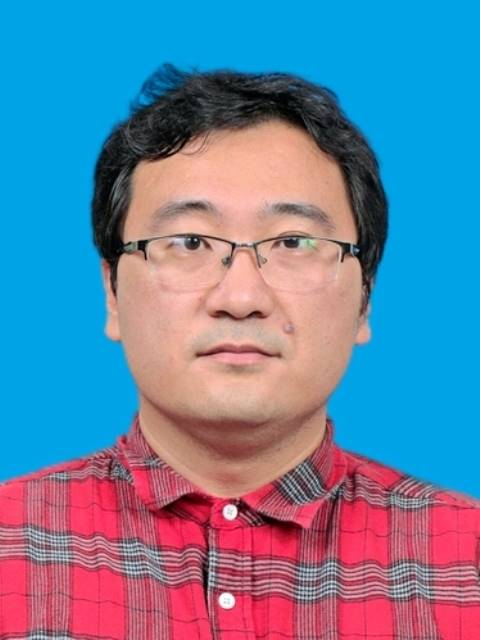
\includegraphics[width=1in,height=1.25in,clip,keepaspectratio]{assets/thales.jpg}}]{Tai Jiang}
  received the master’s degree in Master of Business Administration from the University of Chinese Academy of Sciences, Beijing, in 2022, where he is currently pursuing the Ph.D. degree with the Institute of System Engineering, Macau University of Science and Technology, Macao, China.
  
  he is with the Department of Engineering Science, Faculty of Innovation Engineering, Macau University of Science and Technology, Macao, 999078, China. His research interests include parallel intelligence, blockchain, DAOs, NFTs, Meta, and Decentralized Science.
\end{IEEEbiography}

\vspace{-33pt}

\begin{IEEEbiography}[{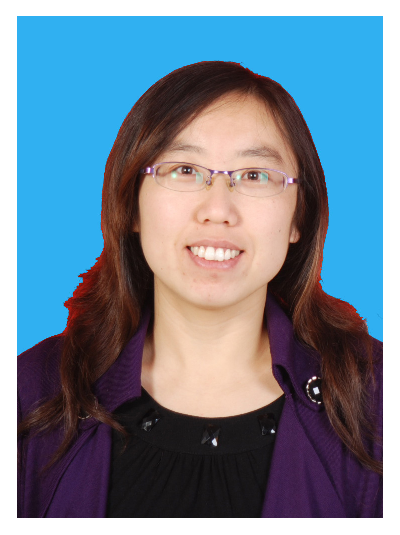
\includegraphics[width=1in,height=1.25in,clip,keepaspectratio]{assets/Rui.eps}}]{Rui Qin}
  (Member, IEEE) received the Ph.D. degree in computer application technology from the University of Chinese Academy of Sciences, Beijing, China, in 2016.

  She is currently an Associate Professor with the State Key Laboratory for Management and Control of Complex Systems, Institute of Automation, Chinese Academy of Sciences, Beijing. Her research interests include blockchain, DAO, and parallel management.
\end{IEEEbiography}

\vspace{-33pt}

\begin{IEEEbiography}[{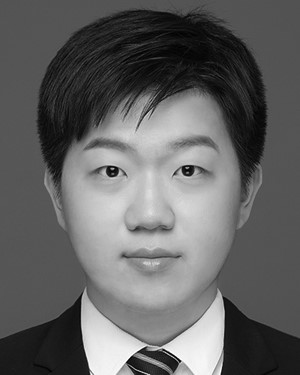
\includegraphics[width=1in,height=1.25in,clip,keepaspectratio]{assets/yhliu.jpg}}]{Yuhang Liu}
  received the B.S. degree from the Department of Precision Instruments, Tsinghua University, Beijing, China, in 2021. He is currently working toward the Ph.D. degree with the Institute of Automation, Chinese Academy of Sciences, Beijing. His research interests include parallel radars, 3D object detection, and point cloud data generation.
\end{IEEEbiography}

\vspace{-33pt}

\begin{IEEEbiography}[{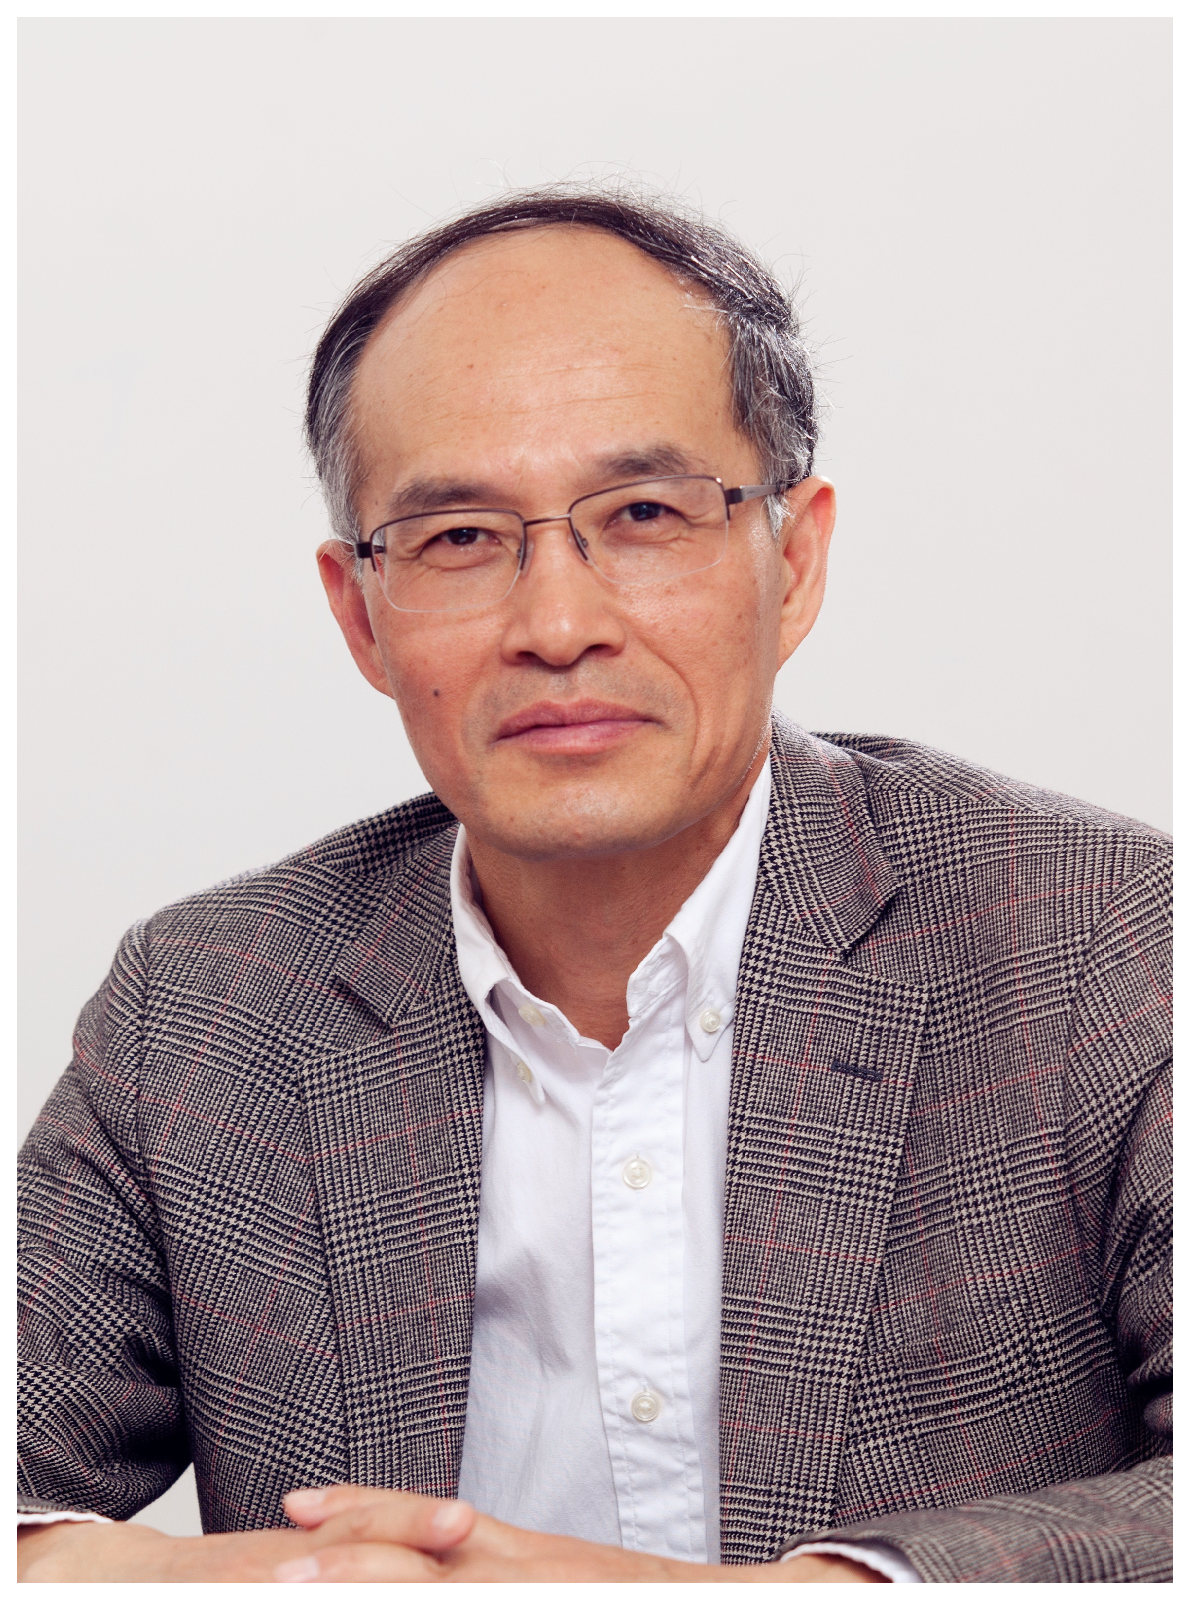
\includegraphics[width=1in,height=1.25in,clip,keepaspectratio]{assets/FW.eps}}]{Fei-Yue Wang} (S’87–M’89–SM’94–F’03)
received his Ph.D. degree in computer and systems engineering from the Rensselaer Polytechnic Institute, Troy, NY, USA, in 1990. He joined The University of Arizona in 1990 and became a Professor and the Director of the Robotics and Automation Laboratory and the Program in Advanced Research for Complex Systems. In 1999, he founded the Intelligent Control and Systems Engineering Center at the Institute of Automation, Chinese Academy of Sciences (CAS), Beijing, China, under the support of the Outstanding Chinese Talents Program from the State Planning Council, and in 2002, was appointed as the Director of the Key Laboratory of Complex Systems and Intelligence Science, CAS, and Vice President of Institute of Automation, CAS in 2006. He found CAS Center for Social Computing and Parallel Management in 2008, and became the State Specially Appointed Expert and the Founding Director of the State Key Laboratory for Management and Control of Complex Systems in 2011. He is a distinguished professor at the Macau University of Science and Technology.

His current research focuses on methods and applications for parallel intelligence, social computing, and knowledge automation. He is a Fellow of International Council on Systems Engineering (INCOSE), International Federation of Automatic Control (IFAC), American Society of Mechanical Engineers (ASME), and American Association for the Advancement of Science (AAAS). In 2007, he received the National Prize in Natural Sciences of China, numerous best papers awards from IEEE Transactions, and became an Outstanding Scientist of Association for Computing Machinery(ACM) for his work in intelligent control and social computing. He received the IEEE Intelligent Transportation Systems (ITS) Outstanding Application and Research Awards in 2009, 2011, and 2015, respectively, the IEEE Systems, Man, and Cybernetics Society (SMC) Norbert Wiener Award in 2014, and became the IFAC Pavel J. Nowacki Distinguished Lecturer in 2021.

Since 1997, he has been serving as the General or Program Chair of over 30 IEEE, Institute for Operations Research and the Management Sciences (INFORMS), IFAC, ACM, and ASME conferences. He was the President of the IEEE ITS Society from 2005 to 2007, the IEEE Council of Radio Frequency Identification (RFID) from 2019 to 2021, the Chinese Association for Science and Technology, USA, in 2005, the American Zhu Kezhen Education Foundation from 2007 to 2008, the Vice President of the ACM China Council from 2010 to 2011, the Vice President and the Secretary General of the Chinese Association of Automation (CAA) from 2008 to 2018, the Vice President of IEEE SMC from 2019 to 2021. He was the Founding Editor-in-Chief (EiC) of the International Journal of Intelligent Control and Systems from 1995 to 2000, IEEE ITS Magazine from 2006 to 2007, JOURNAL OF AUTOMATICA SINICA (IEEE/CAA) from 2014-2017, China's Journal of Command and Control from 2015-2021, and China's Journal of Intelligent Science and Technology from 2019 to 2021. He was the EiC of the IEEE Intelligent Systems from 2009 to 2012, IEEE TRANSACTIONS on ITS from 2009 to 2016, IEEE TRANSACTIONS ON COMPUTATIONAL SOCIAL SYSTEMS from 2017 to 2020. Currently, he is the President of CAA's Supervision Council, and the EiC of IEEE Trans. on Intelligent Vehicles.
\end{IEEEbiography}



\vfill

\end{document}


